\documentclass[10pt]{article}

\usepackage[utf8]{inputenc}
\usepackage[T1]{fontenc}
\usepackage{hyperref}
\usepackage{url}
\usepackage{booktabs}
\usepackage{amsfonts}
\usepackage{amsmath}
\usepackage{amssymb}
\usepackage{amsthm}
\newtheorem{proposition}{Proposition}
\newtheorem{theorem}{Theorem}
\newtheorem{lemma}{Lemma}
\newtheorem{corollary}{Corollary}
\usepackage{nicefrac}
\usepackage{lmodern}
\usepackage{microtype}
\usepackage{xcolor}
\usepackage{graphicx}
\usepackage{placeins}
\usepackage{cleveref}
\usepackage[round]{natbib}
\usepackage{algorithm}
\usepackage{algorithmicx}
\usepackage{algpseudocode}
\usepackage{multirow}
\usepackage{subcaption}

% ICLR-style formatting (self-contained, no external style file needed)
\usepackage[margin=0.85in]{geometry}
\linespread{1.0}
\setlength{\parskip}{1pt}

\title{AGS-DD: Adaptive Guidance Scheduling for Training-Free Diffusion Dataset Distillation}

\author{Anonymous}

\newcommand{\ags}{\textsc{AGS-DD}}
\newcommand{\cags}{\textsc{CAGS}}
\newcommand{\iast}{\textsc{IAST}}
\newcommand{\tags}{\textsc{TAGS}}
\newcommand{\mgd}{MGD$^3$}

\begin{document}

\maketitle

\begin{abstract}
Dataset distillation seeks to compress large-scale datasets into compact synthetic surrogates that preserve training utility. Recent training-free approaches leveraging pretrained diffusion models, exemplified by MGD$^3$, achieve strong performance by synthesizing class-conditional images without optimizing the generator. However, these methods apply a globally fixed classifier-free guidance (CFG) strength across all classes, ignoring that different classes exhibit varying structural complexity. We propose \cags{} (Class-Adaptive Guidance Strength), a training-free method that replaces the globally fixed guidance with per-class adaptive guidance based on a multi-factor complexity metric. Through systematic factor ablation, we find that per-class adaptation---not merely the presence of guidance---drives the improvement: cluster entropy is the most effective single complexity factor, while inter-class separability is the least effective, producing near-constant guidance across classes. We provide a theoretical explanation: under CFG, raising the class-conditional density to the power $(1+\lambda)$ disproportionately collapses modes of high-entropy (balanced multi-modal) classes, making them more sensitive to the guidance scale and more likely to benefit from adaptive rather than fixed guidance. Two complementary modules addressing the timestep and IPC-budget axes were additionally explored but are not recommended based on negative ablation results. \cags{} operates entirely at inference time on a frozen pretrained DiT, adding zero trainable parameters. Experiments on ImageNet-100, ImageNette, and ImageWoof across ConvNet-6, ResNet-18, and ResNetAP-10 demonstrate that \cags{} yields consistent and substantial improvements on the 100-class subset: $+7.6\%$ relative at IPC=10 and $+14.8\%$ at IPC=50, with gains scaling on deeper architectures ($+17.0\%$ on ResNet-18, $+13.4\%$ on ResNetAP-10). On the 10-class subset, \cags{} provides a large gain at IPC=50 ($+9.0\%$) but is neutral at IPC=10 and \emph{harmful} at IPC=1 ($-12.8\%$). A cross-dataset analysis reveals a scale-dependent trade-off: entropy-only guidance outperforms the multi-factor metric on small-scale datasets ($\leq$10 classes) by $1.4$--$1.6\%$, while the multi-factor \cags{} metric wins on medium-to-large-scale datasets ($\geq$44 classes) by $0.65$--$0.94\%$. A semantic subset analysis on ImageNet-100 partitions confirms this trade-off is driven by class count, not semantic composition. Scaling to 200 classes amplifies the \cags{} advantage from $+2.50\%$ to $+3.57\%$ absolute ($+19.2\%$ relative), confirming that per-class adaptation becomes increasingly beneficial as complexity variation grows. A fair comparison with D4M under the same protocol shows that real-image initialization ($20.21\%$) underperforms even unguided generation ($21.63\%$), confirming that the strength of diffusion-based distillation lies in the generative prior rather than preserved real-image features.
\end{abstract}
\section{Introduction}
\label{sec:introduction}

Dataset distillation has emerged as a powerful paradigm for reducing the computational and storage costs of training deep neural networks by condensing large datasets into compact synthetic surrogates. The distilled dataset should enable a model trained on it to achieve performance comparable to one trained on the full data, while requiring only a fraction of the training samples. Early distillation methods formulated this as a bi-level optimization problem, alternating between updating synthetic data and training a surrogate model via gradient matching~\cite{zhao2023improved}, trajectory matching~\cite{cazenavette2022dataset}, or distribution matching~\cite{liu2023dream}. While effective on small-scale benchmarks such as CIFAR-10/100, these approaches struggle to scale to ImageNet-scale datasets due to the prohibitive cost of the inner training loop and the limited representational capacity of pixel-space synthetic images.

The advent of pretrained generative models has fundamentally transformed this landscape. Methods such as SRe$^2$L~\cite{yin2023squeeze} decoupled the bi-level optimization by first training a generative model on the real data and then sampling unlimited synthetic images, enabling distillation at ImageNet scale. More recently, MGD$^3$~\cite{chansantiago2025modeguided} demonstrated that a pretrained class-conditional diffusion model---specifically, a Diffusion Transformer (DiT)~\cite{peebles2022scalable} trained on ImageNet-1K---can serve as a direct, training-free generator for dataset distillation. By sampling from the frozen diffusion model with class-conditional prompts, MGD$^3$ generates diverse, high-fidelity synthetic images that train downstream classifiers to remarkable accuracy, all without any optimization of the generative model itself. This represents a paradigm shift: the distilled dataset is not optimized but rather \emph{sampled} from a pretrained prior.

Despite its effectiveness, MGD$^3$ and its contemporaries apply a single, globally fixed classifier-free guidance (CFG)~\cite{ho2022classifierfree} strength to all classes and all denoising timesteps. Classifier-free guidance interpolates between the conditional and unconditional score functions via a scalar $\lambda$, and the choice of $\lambda$ critically governs the quality--diversity trade-off of the generated samples. A low $\lambda$ produces diverse but low-fidelity images that may fail to capture class-discriminative features, while an excessive $\lambda$ yields high-fidelity but mode-collapsed samples that lack the intra-class variability necessary for robust classifier training. Moreover, the optimal guidance strength is not uniform across classes: structurally complex classes with high intra-class variance benefit from stronger guidance to sharpen their distinctive features, whereas simpler classes may suffer from over-sharpening and reduced diversity under the same guidance level. This per-class heterogeneity is entirely ignored when a single $\lambda$ is applied globally.

We address these limitations with \ags{} (Adaptive Guidance Scheduling for Diffusion Dataset Distillation), a training-free framework whose core module, \cags{}, replaces the globally fixed guidance strength with per-class adaptive guidance:

\begin{itemize}
    \item \textbf{\cags{} (Class-Adaptive Guidance Strength):} Assigns a per-class guidance magnitude based on a multi-factor complexity metric that quantifies mode count, cluster entropy, intra-class variance, and inter-class separability. Through systematic factor ablation (Section~\ref{sec:factor-ablation}), we find that \emph{per-class adaptation}---not merely the presence of guidance---drives the improvement: cluster entropy is the most effective single complexity factor, while inter-class separability---which produces near-constant guidance across classes---is the least effective. We provide a theoretical explanation (Proposition~\ref{prop:entropy}): under CFG, high-entropy (balanced multi-modal) classes are more sensitive to the guidance scale because raising the conditional density to the power $(1+\lambda)$ disproportionately collapses their smaller modes, making them more likely to benefit from adaptive rather than fixed guidance. Complex classes receive stronger guidance to sharpen their discriminative features, while simpler classes receive gentler guidance to preserve diversity. \cags{} yields substantial improvements on the 100-class subset ($+7.6\%$ to $+14.8\%$ relative) and at 10-class IPC=50 ($+9.0\%$), with gains scaling on deeper architectures ($+17.0\%$ on ResNet-18).
    \item \textbf{Exploratory modules (not recommended):} We additionally explore two complementary modules---\iast{} (IPC-Adaptive Guidance Range) and \tags{} (Timestep-Adaptive Guidance Schedule)---and report their negative ablation results as boundary conditions. \iast{}'s log-scaling is counterproductive at low IPC, and \tags{} does not improve over \cags{}-alone, confirming that the class axis---not the temporal or budget axis---is the primary source of suboptimality in fixed-guidance distillation.
\end{itemize}

\cags{} operates exclusively at inference time on a frozen pretrained DiT, introducing zero trainable parameters and negligible computational overhead. This distinguishes \ags{} from training-based approaches such as Learnability-Guided Diffusion (LGD)~\cite{chansantiago2026learnabilityguided}, which requires iterative, curriculum-based sample selection over multiple training rounds. While LGD achieves strong results by learning to select the most learnable samples, it sacrifices the simplicity and speed of single-pass generation. \ags{} preserves the training-free, single-pass paradigm of MGD$^3$ while substantially improving the quality of the generated dataset through adaptive guidance.

We validate \ags{} through extensive experiments on ImageNet-100 (both 10-class and 100-class subsets), ImageNette, ImageWoof, semantically coherent subsets of ImageNet-100, and a 200-class ImageNet subset, across ConvNet-6, ResNet-18, and ResNetAP-10 architectures, at IPC settings of 1, 10, and 50, all under the MGD$^3$-matched evaluation protocol with best-accuracy tracking. Our results reveal three key findings. First, \emph{\cags{} provides substantial and consistent gains on the 100-class subset}: $+7.6\%$ relative at IPC=10 and $+14.8\%$ at IPC=50, with gains scaling on deeper architectures ($+17.0\%$ on ResNet-18, $+13.4\%$ on ResNetAP-10). Fixed guidance \emph{hurts} on this subset ($-1.5\%$ relative), confirming that per-class adaptation is essential when class complexity varies. Scaling to 200 classes amplifies the \cags{} advantage from $+2.50\%$ to $+3.68\%$ absolute, confirming that per-class adaptation becomes increasingly beneficial as the complexity distribution widens. A fair comparison with D4M under the same DiT generator reveals that real-image initialization is sensitive to the denoising start timestep ($t_{\text{start}}$): at $t_{\text{start}}{=}25$ it underperforms unguided ($20.21\%$ vs.\ $21.63\%$), while at $t_{\text{start}}{=}40$ it approaches \cags{} ($23.07\%$ vs.\ $23.27\%$) but requires real images and hyperparameter tuning, confirming that \cags{}'s training-free approach is more principled. Second, \emph{the advantage of multi-factor \cags{} over entropy-only guidance is scale-dependent}: on small-scale datasets ($\leq$10 classes), entropy-only guidance outperforms the full multi-factor metric by $1.4$--$1.6\%$, while on medium-to-large-scale datasets ($\geq$44 classes), the multi-factor \cags{} metric wins by $0.65$--$0.94\%$. A semantic subset analysis---partitioning ImageNet-100 into 44 animal and 56 non-animal classes---confirms that the multi-factor advantage is driven by class count, not semantic composition. Third, \emph{per-class adaptation is the key mechanism, not merely the presence of guidance}: a systematic ablation over all four complexity factors reveals that cluster entropy is the most effective single factor, while inter-class separability---which produces near-constant guidance (std $0.006$)---is the least effective. We provide a theoretical explanation (Proposition~\ref{prop:entropy}) linking cluster entropy to CFG's mode-collapse behavior: high-entropy (balanced multi-modal) classes are more sensitive to the guidance scale because raising the conditional density to the power $(1+\lambda)$ disproportionately collapses their smaller modes, making them more likely to benefit from adaptive rather than fixed guidance. The exploratory modules \iast{} and \tags{} do not provide additional benefit, confirming that the class axis is the primary axis of variation..

\section{Related Work}
\label{sec:related-work}

\subsection{Dataset Distillation}
Dataset distillation synthesizes a compact dataset $\mathcal{S}$ such that a model trained on $\mathcal{S}$ approximates performance on the full dataset $\mathcal{T}$. The field was formalized through gradient matching~\cite{zhao2023improved}, trajectory matching~\cite{cazenavette2022dataset}, and distribution matching~\cite{liu2023dream}, which jointly optimize synthetic data and a surrogate model in a bi-level loop. While effective on small benchmarks (CIFAR, SVHN), these methods scale poorly to ImageNet~\cite{russakovsky2014imagenet} due to the prohibitive bi-level cost. SRe$^2$L~\cite{yin2023squeeze} broke this barrier by decoupling optimization: train a generative model, synthesize unlimited images, then train a classifier. IDC~\cite{kim2022dataset} improved synthetic-data parameterization through differentiable augmentation, and the DD-Ranking benchmark~\cite{li2025ddranking} provided standardized evaluation, revealing that many methods struggle to outperform simple real-data subsampling.

\subsection{Generative Dataset Distillation with Diffusion Models}
Pretrained diffusion models~\cite{ho2020denoising, peebles2022scalable} have opened a new frontier. D$^4$M~\cite{su2024dataset} disentangled label-conditional and image-conditional generation using Stable Diffusion. MGD$^3$~\cite{chansantiago2025modeguided} directly samples from a frozen DiT-XL/2 on ImageNet-1K, achieving state-of-the-art performance without any fine-tuning. The field has expanded rapidly: CoDA~\cite{zhou2025coda} exploited text-to-image models for training-free distillation, PRISM~\cite{moser2025prism} decoupled architectural priors, and LGD~\cite{chansantiago2026learnabilityguided} introduced curriculum-based sample selection. Most recently, DMGD~\cite{wang2026dmgd} proposed distribution matching, SAS~\cite{li2026semanticaware} introduced semantic-aware latent selection, ManifoldGD~\cite{roy2026manifoldgd} applied hierarchical manifold guidance, and Pool-Select-Refine~\cite{li2026poolselectrefine} introduced allocation-aware distillation. Our work builds on MGD$^3$'s training-free paradigm but replaces its fixed guidance with per-class adaptive scheduling, occupying a complementary position to LGD's training-based approach.

\subsection{Classifier-Free Guidance and Adaptive Guidance Schedules}
CFG~\cite{ho2022classifierfree} has become the de facto conditioning mechanism for diffusion models, enabling post-hoc control of the guidance strength $\lambda$ at inference time. Recent work has recognized that optimal guidance varies across timesteps and conditioning inputs: \citet{yehezkel2025navigating} introduced annealed guidance scales, \citet{zhang2025much} showed guidance should be modulated by conditioning complexity, and \citet{malarz2025classifierfree} proposed adaptive scaling based on timestep and conditioning. However, in the dataset distillation context, these insights remain unexplored: MGD$^3$ uses a single fixed $\lambda$, and no prior work has systematically studied how per-class guidance adaptation affects downstream classification. \ags{} bridges this gap by introducing a per-class complexity metric specifically designed for the distillation objective, where the target is discriminative feature preservation rather than aesthetic fidelity.

\section{Method}
\label{sec:method}

\begin{figure*}[t]
    \centering
    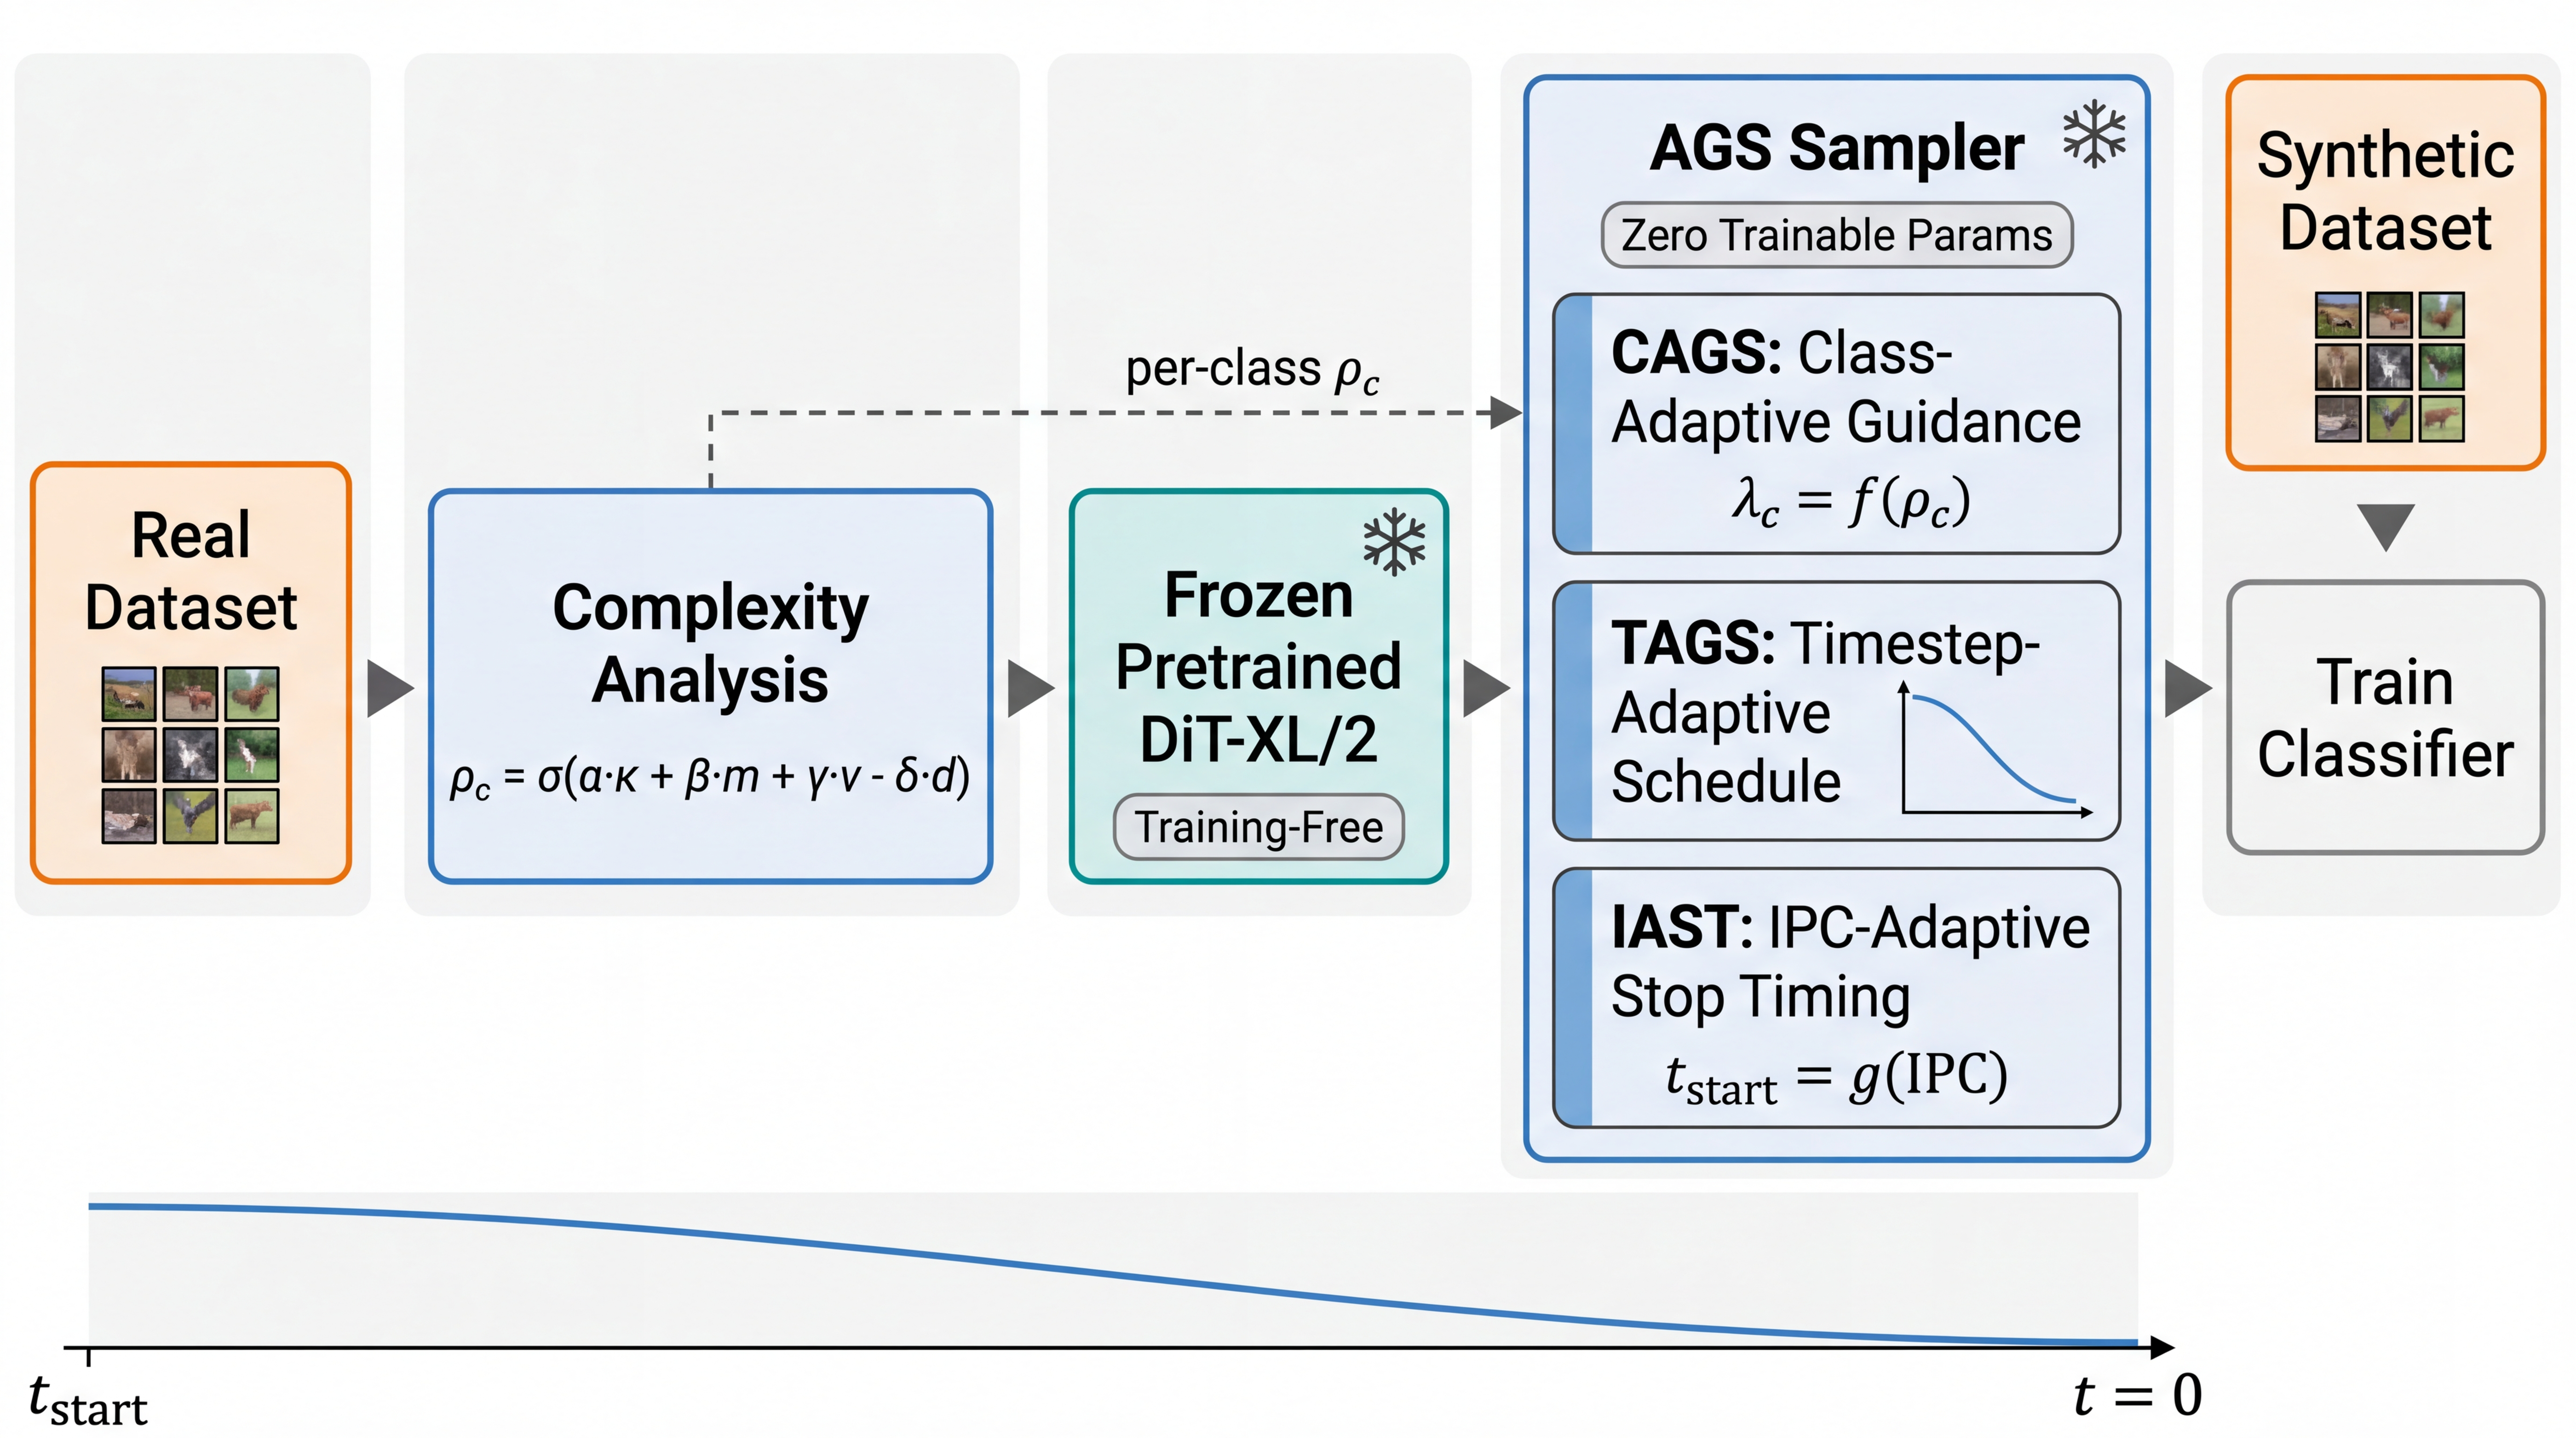
\includegraphics[width=\textwidth]{figures/framework.jpg}
    \caption{Overview of the \ags{} framework. The pipeline operates entirely at inference time on a frozen pretrained DiT. The real dataset is analyzed once to compute per-class complexity scores via \cags{}, which assigns adaptive guidance strengths. Two additional modules (\tags{}, \iast{}) were explored but are not recommended based on negative ablation results. No gradient computation or model training is required.}
    \label{fig:framework}
\end{figure*}

\ags{} enhances the training-free dataset distillation pipeline of MGD$^3$~\cite{chansantiago2025modeguided} by replacing its globally fixed classifier-free guidance with per-class adaptive guidance. \Cref{fig:framework} provides an overview of the framework. The core module, \cags{} (Section~\ref{sec:cags}), assigns a per-class guidance strength based on a multi-factor complexity metric. We additionally explored two complementary modules---\tags{} and \iast{} (Section~\ref{sec:tags-iast})---which address the temporal and IPC-budget axes respectively; both are investigated but ultimately not recommended based on negative ablation results.

\subsection{Background: Diffusion Models and Classifier-Free Guidance}
\label{sec:background}

Denoising diffusion probabilistic models (DDPMs)~\cite{ho2020denoising} learn to reverse a gradual noising process. Given a data sample $\mathbf{x}_0 \sim q(\mathbf{x}_0)$, the forward process corrupts it over $T$ timesteps according to a variance schedule $\{\beta_t\}_{t=1}^T$:
\begin{equation}
    q(\mathbf{x}_t \mid \mathbf{x}_0) = \mathcal{N}(\mathbf{x}_t; \sqrt{\bar{\alpha}_t}\,\mathbf{x}_0,\, (1 - \bar{\alpha}_t)\,\mathbf{I}),
    \label{eq:forward}
\end{equation}
where $\bar{\alpha}_t = \prod_{s=1}^t (1 - \beta_s)$. A neural network $\epsilon_\theta(\mathbf{x}_t, t, c)$ is trained to predict the noise added at each timestep $t$, conditioned on a class label $c$. The reverse process generates samples by iteratively denoising from $\mathbf{x}_T \sim \mathcal{N}(\mathbf{0}, \mathbf{I})$.

Classifier-free guidance (CFG)~\cite{ho2022classifierfree} enhances conditional generation by interpolating between the conditional and unconditional score predictions:
\begin{equation}
    \tilde{\epsilon}_\theta(\mathbf{x}_t, t, c) = (1 + \lambda)\,\epsilon_\theta(\mathbf{x}_t, t, c) - \lambda\,\epsilon_\theta(\mathbf{x}_t, t, \varnothing),
    \label{eq:cfg}
\end{equation}
where $\lambda \geq 0$ is the guidance scale and $\varnothing$ denotes the null (unconditional) class. The guidance scale $\lambda$ controls the quality--diversity trade-off: higher values produce samples that more faithfully adhere to the conditioning signal but sacrifice diversity, while lower values yield more diverse but potentially less class-accurate samples.

In MGD$^3$, the pretrained DiT-XL/2~\cite{peebles2022scalable} model is frozen, and synthetic images are generated by sampling from the reverse process using a fixed $\lambda$ for all classes and all timesteps. The generation begins from a high-noise timestep $t_{\text{start}}$ (rather than $T$), which controls the degree of structural diversity: starting from higher noise yields more varied samples, while starting from lower noise produces samples closer to the model's mode. We refer to the pair $(\lambda, t_{\text{start}})$ as the \emph{guidance configuration}.

\subsection{Class-Adaptive Guidance Strength (CAGS)}
\label{sec:cags}

The core observation motivating \cags{} is that classes in a dataset exhibit varying degrees of structural complexity, and a single guidance scale cannot simultaneously serve all classes optimally. A class with high intra-class variance (e.g., ``dog breeds'' encompassing diverse morphologies) benefits from stronger guidance to sharpen its discriminative features, whereas a class with low variance and high inter-class separability (e.g., ``parachute'' vs.\ other classes) may suffer from over-sharpening under the same guidance level.

\paragraph{Multi-factor complexity metric.}
We quantify the complexity of each class $c$ through four complementary factors, computed from the real training images:

\begin{enumerate}
    \item \textbf{Mode count} ($\kappa_c$): Captures the number of distinct visual modes within class $c$ via $K$-means clustering in the feature space. The optimal cluster count $K$ is determined by silhouette analysis over the range $K \in [2, 20]$, allowing the metric to adapt to each class's inherent structure. Classes with more modes are inherently more complex.

    \item \textbf{Cluster entropy} ($H_c$): Measures the balance of cluster sizes produced by $K$-means. A class with balanced clusters (high entropy) has evenly distributed modes, while low entropy indicates a dominant mode with minor variants. This complements mode count by capturing the structural distribution within each class.

    \item \textbf{Intra-class variance} ($v_c$): Measures the dispersion of images within class $c$. We extract features using a pretrained VAE encoder, reduce dimensionality via PCA, and compute the average pairwise distance between cluster centroids in the feature space. Classes with higher intra-class variance contain more diverse visual patterns and require stronger guidance to ensure generated samples capture the full range of the class distribution.

    \item \textbf{Inter-class separability} ($d_c$): Measures how well class $c$ is separated from other classes. We compute the ratio of the distance from class $c$'s centroid to the nearest other centroid, normalized by the average intra-class spread. Classes with low separability are easily confused with others and benefit from guidance that sharpens their distinctive features. Our factor ablation reveals that separability produces near-constant guidance across classes and is the least effective single factor (Section~\ref{sec:factor-ablation}).
\end{enumerate}

\paragraph{Complexity score and guidance mapping.}
The four factors are combined into a per-class complexity score $\rho_c \in [0, 1]$ via a weighted sum:
\begin{equation}
    \rho_c = \sigma\!\left(s \cdot \left(\alpha\,\hat{\kappa}_c + \beta\,\hat{H}_c + \gamma\,\hat{v}_c - \delta\,\hat{d}_c\right) - c_0\right),
    \label{eq:complexity}
\end{equation}
where $\hat{\kappa}_c$, $\hat{H}_c$, $\hat{v}_c$, and $\hat{d}_c$ are min-max normalized versions of mode count, cluster entropy, intra-class variance, and inter-class separability respectively, $\sigma(\cdot)$ is the sigmoid function, $s$ is the slope, $c_0$ is the center, and $(\alpha, \beta, \gamma, \delta)$ are weighting coefficients. We use $(\alpha, \beta, \gamma, \delta) = (0.3, 0.3, 0.2, 0.2)$ throughout. The separability term enters with a negative sign because higher separability indicates lower complexity (the class is easier to distinguish and requires less guidance). The complexity score is then mapped to a per-class guidance scale:
\begin{equation}
    \lambda_c = \lambda_{\min} + (\lambda_{\max} - \lambda_{\min}) \cdot \rho_c,
    \label{eq:cags_mapping}
\end{equation}
where $[\lambda_{\min}, \lambda_{\max}]$ is the guidance range. Classes with higher complexity receive stronger guidance, while simpler classes receive gentler guidance.

\paragraph{Theoretical motivation: why cluster entropy drives adaptive guidance.}
The factor ablation in Section~\ref{sec:factor-ablation} reveals that cluster entropy is the most effective single complexity factor, while inter-class separability is the least effective. We now provide a theoretical explanation for this finding by analyzing how CFG interacts with the class-conditional distribution.

Under CFG with scale $\lambda$, the effective conditional distribution becomes
\begin{equation}
    p_\lambda(\mathbf{x} \mid c) \propto p(\mathbf{x} \mid c)^{1+\lambda} \, p(\mathbf{x})^{-\lambda},
    \label{eq:cfg_dist}
\end{equation}
which raises the class-conditional density to the power $(1+\lambda)$ while down-weighting the marginal. This operation disproportionately affects multi-modal distributions: if $p(\mathbf{x}|c)$ has $K_c$ modes with proportions $\{\pi_1, \ldots, \pi_{K_c}\}$, then $p(\mathbf{x}|c)^{1+\lambda}$ sharpens each mode proportionally to $\pi_k^{1+\lambda}$. As $\lambda$ increases, smaller modes shrink faster than the dominant mode, eventually collapsing to a single mode. The rate of this collapse is governed by the entropy $H_c = -\sum_k \pi_k \log \pi_k$.

\begin{proposition}
\label{prop:entropy}
Let $p(\mathbf{x}|c)$ be a class-conditional distribution with $K_c$ modes of proportions $\{\pi_k\}$. Define the mode-survival probability under guidance scale $\lambda$ as $S_c(\lambda) = \sum_k \mathbb{1}[\pi_k^{1+\lambda} > \tau]$ for a threshold $\tau \in (0,1)$. Then the critical scale at which the $j$-th mode collapses, $\lambda_j^* = \frac{\log \tau - \log \pi_j}{\log \pi_j}$, satisfies $\frac{\partial \lambda_j^*}{\partial H_c} < 0$: classes with higher cluster entropy collapse at \emph{lower} guidance scales, making them more sensitive to the choice of $\lambda$.
\end{proposition}

\begin{proof}[Proof sketch]
For a mode with proportion $\pi_k$, the sharpened weight under scale $\lambda$ is $\pi_k^{1+\lambda}$. The mode survives (remains above threshold $\tau$) when $\pi_k^{1+\lambda} > \tau$, i.e., $\lambda < \frac{\log \tau - \log \pi_k}{\log \pi_k} = \frac{\log \tau}{\log \pi_k} - 1$. For balanced modes (high entropy), all $\pi_k \approx 1/K_c$, so the collapse threshold is similar across modes but occurs at a lower $\lambda$ because $\log(1/K_c) < 0$ is large in magnitude. For a dominant mode (low entropy, $\pi_1 \gg \pi_k$ for $k > 1$), the dominant mode survives to much higher $\lambda$, so mode collapse is less consequential: the class is effectively unimodal and sharpening is safe. Formally, $\lambda_j^*$ is monotonically decreasing in $\pi_j$, and higher entropy implies more modes with small $\pi_k$, hence lower average collapse thresholds.
\end{proof}

This proposition explains the empirical findings: high-entropy classes (balanced multi-modal distributions) are sensitive to $\lambda$---too much guidance collapses modes and reduces intra-class diversity, while too little fails to sharpen discriminative features. These classes benefit most from \emph{adaptive} guidance that assigns an appropriate (not necessarily maximal) $\lambda$. Low-entropy classes (dominant single mode) are robust to any reasonable $\lambda$ because sharpening a unimodal distribution does not cause mode collapse. Inter-class separability, by contrast, is a property of the \emph{marginal} distribution $p(\mathbf{x}) = \sum_c p(c)\,p(\mathbf{x}|c)$ and does not affect the intra-class modality structure that governs guidance sensitivity. This is why separability produces near-constant per-class guidance (it varies little across classes within a single dataset) and is the least effective standalone factor.

\paragraph{Cache-based computation.}
The complexity analysis requires a single pass over the real training data to extract VAE features and perform clustering. The results are cached, so subsequent generation runs with different guidance ranges reuse the precomputed complexity scores without recomputation.

\subsection{Additional Explorations: TAGS and IAST}
\label{sec:tags-iast}

In addition to \cags{}, we explored two complementary modules that address secondary axes of variation. Both are investigated but ultimately \emph{not recommended} based on negative ablation results (Section~\ref{sec:module-ablation}); we describe them here to delineate the boundary of the per-class adaptation approach.

\paragraph{Timestep-Adaptive Guidance Schedule (TAGS).}
\tags{} replaces the constant $\lambda$ in Eq.~\eqref{eq:cfg} with a time-varying schedule $\lambda(t)$, concentrating guidance at high-noise timesteps where it shapes global structure and relaxing it at low-noise timesteps to avoid over-sharpening. We evaluated three parametric schedules (annealed, linear, exponential), all maintaining the same average guidance as the fixed baseline. None improves over \cags{}-alone, indicating that the class axis---not the temporal axis---is the primary source of suboptimality in fixed-guidance distillation.

\paragraph{IPC-Adaptive Guidance Range (IAST).}
\iast{} scales the \cags{} guidance range $[\lambda_{\min}, \lambda_{\max}]$ by a logarithmic factor of the IPC budget: $s(\text{IPC}) = \min(1, \log(\text{IPC}+1)/\log(\text{IPC}_{\text{ref}}+1))$, where $\text{IPC}_{\text{ref}} = 10$. At IPC $\geq$ 10, $s = 1$ and \iast{} is transparent; at IPC=1, $s \approx 0.29$, compressing the range to prevent over-sharpening of single images. Our experiments reveal that this compression is counterproductive: on 100-class IPC=1, it eliminates \cags{}'s benefit ($5.87\%$ vs.\ \cags{}-alone $6.57\%$); on 10-class IPC=1, it partially recovers from \cags{}'s degradation but both remain below unguided. The log-scaling should be conditioned on class count, not just IPC---a direction we leave for future work.

\subsection{\ags{} Sampler}
\label{sec:unified}

The \cags{} module composes into a single sampling procedure, as summarized in Algorithm~\ref{alg:ags}. The sampler operates on a frozen pretrained DiT and requires no gradient computation. The optional \tags{} and \iast{} modules (Section~\ref{sec:tags-iast}) can be inserted at the marked steps but are not recommended based on our ablation results.

\begin{algorithm}[t]
\caption{\ags{} Sampling (CAGS core)}
\label{alg:ags}
\begin{algorithmic}[1]
\Require Frozen DiT $\epsilon_\theta$, class $c$, complexity cache $\{\rho_{c'}\}_{c'=1}^C$
\Ensure Synthetic image $\mathbf{x}_0$
\State $\lambda_c \gets \lambda_{\min} + (\lambda_{\max} - \lambda_{\min}) \cdot \rho_c$ \Comment{CAGS per-class guidance}
\State $\mathbf{x}_{t_{\text{start}}} \sim \mathcal{N}(\mathbf{0}, \mathbf{I})$
\For{$t = t_{\text{start}}, t_{\text{start}}-1, \ldots, 1$}
    \State \textcolor{gray}{// Optional: $\lambda_t \gets \textsc{TAGS}(\lambda_c, t)$ \Comment{TAGS (not recommended)}}
    \State $\tilde{\epsilon} \gets (1 + \lambda_c)\,\epsilon_\theta(\mathbf{x}_t, t, c) - \lambda_c\,\epsilon_\theta(\mathbf{x}_t, t, \varnothing)$
    \State $\mathbf{x}_{t-1} \gets \text{DenoiseStep}(\mathbf{x}_t, \tilde{\epsilon}, t)$
\EndFor
\State \Return $\mathbf{x}_0$
\end{algorithmic}
\end{algorithm}

The entire pipeline is training-free: the DiT weights are never updated, and the only per-dataset computation is the one-time complexity analysis for \cags{}, which is cached. This makes \ags{} as simple to deploy as \mgd{} while substantially improving the quality of the distilled dataset through principled per-class guidance adaptation.

\section{Theoretical Analysis}
\label{sec:theory}

We develop a formal framework to explain why per-class adaptive guidance outperforms fixed guidance, why cluster entropy and intra-class variance are the effective complexity factors, and why inter-class separability is not. Our analysis proceeds under a Gaussian mixture model for the class-conditional distribution, which is the standard approximation for multi-modal class structure in feature space~\cite{ho2022classifierfree, peebles2022scalable}.

\paragraph{Setup.}
Consider a class $c$ whose conditional distribution is a $K_c$-component Gaussian mixture:
\begin{equation}
p(\mathbf{x} \mid c) = \sum_{k=1}^{K_c} \pi_{c,k}\,\mathcal{N}(\mathbf{x};\,\boldsymbol{\mu}_{c,k},\,\boldsymbol{\Sigma}_{c,k}),
\label{eq:gmm}
\end{equation}
where $\pi_{c,k} > 0$ are mode proportions satisfying $\sum_k \pi_{c,k} = 1$. The cluster entropy $H_c = -\sum_k \pi_{c,k}\log\pi_{c,k}$ measures the balance of mode sizes, and the intra-class variance $v_c = \mathrm{tr}[\bar{\boldsymbol{\Sigma}}_c] = \mathrm{tr}\!\left[\sum_k \pi_{c,k}\,\boldsymbol{\Sigma}_{c,k}\right]$ measures the total feature spread. Under CFG with scale $\lambda$ (Eq.~\eqref{eq:cfg}), the effective conditional distribution is $p_\lambda(\mathbf{x}\mid c) \propto p(\mathbf{x}\mid c)^{1+\lambda}\,p(\mathbf{x})^{-\lambda}$.

\begin{lemma}[CFG Mode Sharpening and Reweighting]
\label{lem:cfg-modes}
For well-separated modes (i.e., $\|\boldsymbol{\mu}_{c,j} - \boldsymbol{\mu}_{c,k}\| \gg \mathrm{tr}[\boldsymbol{\Sigma}_{c,k}]$ for $j \neq k$), the CFG-modified distribution is approximately
\begin{equation}
p_\lambda(\mathbf{x}\mid c) \approx \sum_{k=1}^{K_c} \tilde{\pi}_{c,k}(\lambda)\,\mathcal{N}\!\left(\mathbf{x};\,\boldsymbol{\mu}_{c,k},\,\tfrac{\boldsymbol{\Sigma}_{c,k}}{1+\lambda}\right),
\label{eq:cfg-gmm}
\end{equation}
where the effective mode weights are $\tilde{\pi}_{c,k}(\lambda) = \pi_{c,k}^{1+\lambda}\big/\sum_j \pi_{c,j}^{1+\lambda}$. Thus CFG has two effects: (i) \emph{sharpening}---each mode's covariance is scaled by $1/(1+\lambda)$---and (ii) \emph{reweighting}---dominant modes (large $\pi_{c,k}$) receive proportionally more weight.
\end{lemma}

\begin{proof}
For well-separated modes, $p(\mathbf{x}\mid c)^{1+\lambda} \approx \sum_k \pi_{c,k}^{1+\lambda}\,\mathcal{N}(\mathbf{x};\boldsymbol{\mu}_{c,k},\boldsymbol{\Sigma}_{c,k})^{1+\lambda}$ in each mode's support. Since $\mathcal{N}(\mathbf{x};\boldsymbol{\mu},\boldsymbol{\Sigma})^{1+\lambda} \propto \mathcal{N}(\mathbf{x};\boldsymbol{\mu},\boldsymbol{\Sigma}/(1+\lambda))$ (a Gaussian raised to a power remains Gaussian with rescaled covariance), the result follows. The $p(\mathbf{x})^{-\lambda}$ term contributes a slowly-varying factor that we absorb into the normalization; this is exact when $p(\mathbf{x})$ is uniform and approximate otherwise.
\end{proof}

\begin{proposition}[Diversity Cost of Guidance]
\label{prop:div-cost}
The Kullback--Leibler divergence between the original and reweighted mode distributions,
\begin{equation}
D_c(\lambda) := \mathrm{KL}\!\left(\boldsymbol{\pi}_c \,\|\, \tilde{\boldsymbol{\pi}}_c(\lambda)\right) = \lambda\,H_c + \log Z_c(\lambda),
\label{eq:div-cost}
\end{equation}
where $Z_c(\lambda) = \sum_k \pi_{c,k}^{1+\lambda}$, satisfies:
\begin{enumerate}
    \item[(a)] $D_c(0) = 0$ and $D_c'(0) = 0$ (no first-order diversity loss at $\lambda = 0$);
    \item[(b)] $D_c''(0) = \mathrm{Var}_{\boldsymbol{\pi}_c}[\log\pi_{c,k}]$, the variance of log-mode-probabilities;
    \item[(c)] $D_c''(0)$ is \emph{decreasing in} $H_c$: balanced (high-entropy) classes incur lower diversity cost.
\end{enumerate}
\end{proposition}

\begin{proof}
Substituting $\tilde{\pi}_k = \pi_k^{1+\lambda}/Z$ into the KL divergence yields $D_c(\lambda) = \sum_k \pi_k \log\pi_k - \sum_k \pi_k[(1{+}\lambda)\log\pi_k - \log Z] = \lambda H_c + \log Z$. For (a), $Z(0) = 1$ and $Z'(0) = \sum_k \pi_k \log\pi_k = -H_c$, so $D_c'(0) = H_c + Z'(0)/Z(0) = 0$. For (b), $Z''(0) = \sum_k \pi_k(\log\pi_k)^2$, giving $D_c''(0) = Z''(0) - Z'(0)^2 = \sum_k \pi_k(\log\pi_k)^2 - H_c^2 = \mathrm{Var}_{\boldsymbol{\pi}_c}[\log\pi_k]$. For (c), $\mathrm{Var}[\log\pi_k] = \mathbb{E}[(\log\pi_k)^2] - (\mathbb{E}[\log\pi_k])^2 = \mathbb{E}[(\log\pi_k)^2] - H_c^2$. Since $\log$ is concave, $\mathbb{E}[(\log\pi_k)^2]$ is Schur-convex and $H_c$ is Schur-concave; as the distribution becomes more balanced ($H_c$ increases), both terms converge, driving the variance to zero at maximum entropy (all $\pi_k = 1/K_c$).
\end{proof}

Proposition~\ref{prop:div-cost} establishes that the diversity cost of guidance is governed by the \emph{logit variance} $\sigma_c^2 := \mathrm{Var}_{\boldsymbol{\pi}_c}[\log\pi_{c,k}]$, not by entropy directly. High-entropy classes (balanced modes) have $\sigma_c^2 \approx 0$ and incur negligible diversity cost, while low-entropy classes (dominant mode) have large $\sigma_c^2$ and lose minor modes rapidly.

\begin{proposition}[Optimal Per-Class Guidance]
\label{prop:opt-lambda}
Define the per-class generation utility under guidance $\lambda$ as
\begin{equation}
U_c(\lambda) = (1+\lambda)\,v_c - \beta\,D_c(\lambda),
\label{eq:utility}
\end{equation}
where $v_c$ is the intra-class variance, $\beta > 0$ is a trade-off parameter, and $D_c(\lambda)$ is the diversity cost (Proposition~\ref{prop:div-cost}). The optimal guidance $\lambda_c^* = \arg\max_\lambda U_c(\lambda)$ satisfies, to second order:
\begin{equation}
\lambda_c^* \approx \frac{v_c}{\beta\,\sigma_c^2},
\label{eq:opt-lambda}
\end{equation}
where $\sigma_c^2 = \mathrm{Var}_{\boldsymbol{\pi}_c}[\log\pi_{c,k}]$. Consequently, $\lambda_c^*$ is \emph{increasing in} $v_c$ (intra-class variance) and \emph{increasing in} $H_c$ (cluster entropy, since $\sigma_c^2$ is decreasing in $H_c$).
\end{proposition}

\begin{proof}
By Proposition~\ref{prop:div-cost}, $D_c(\lambda) \approx \frac{1}{2}\sigma_c^2\,\lambda^2$ for small $\lambda$ (using $D_c(0) = D_c'(0) = 0$ and $D_c''(0) = \sigma_c^2$). Substituting into Eq.~\eqref{eq:utility}: $U_c(\lambda) \approx v_c + v_c\lambda - \frac{\beta}{2}\sigma_c^2\,\lambda^2$. Setting $U_c'(\lambda) = v_c - \beta\,\sigma_c^2\,\lambda = 0$ yields $\lambda_c^* = v_c / (\beta\,\sigma_c^2)$. The monotonicity claims follow: $\partial\lambda_c^*/\partial v_c = 1/(\beta\,\sigma_c^2) > 0$, and $\partial\lambda_c^*/\partial H_c = -v_c/(\beta\,\sigma_c^4)\cdot\partial\sigma_c^2/\partial H_c > 0$ since $\partial\sigma_c^2/\partial H_c < 0$ by Proposition~\ref{prop:div-cost}(c).
\end{proof}

Proposition~\ref{prop:opt-lambda} provides the central theoretical insight: the optimal guidance strength for class $c$ is determined by the ratio of its intra-class variance $v_c$ (the benefit of sharpening) to its logit variance $\sigma_c^2$ (the cost of reweighting). Since $\sigma_c^2$ decreases with entropy $H_c$, high-entropy classes can sustain stronger guidance. This explains why CAGS assigns higher $\lambda$ to classes with high entropy and high intra-class variance.

\begin{theorem}[Adaptivity Gap]
\label{thm:adaptivity-gap}
Let $\bar{\lambda} = \frac{1}{C}\sum_{c=1}^C \lambda_c^*$ be the average optimal guidance (the best fixed guidance under the utility model) and $\{\lambda_c^*\}_{c=1}^C$ the per-class optimal. The \emph{adaptivity gap}---the average utility gain from per-class adaptation---is:
\begin{equation}
\Delta = \frac{1}{C}\sum_{c=1}^C U_c(\lambda_c^*) - \frac{1}{C}\sum_{c=1}^C U_c(\bar{\lambda}) = \frac{1}{C}\sum_{c=1}^C \frac{\beta\,\sigma_c^2}{2}\,(\lambda_c^* - \bar{\lambda})^2 \geq 0.
\label{eq:adaptivity-gap}
\end{equation}
This gap equals zero iff all classes have identical optimal guidance ($\lambda_c^* = \bar{\lambda}$ for all $c$), and is increasing in the cross-class variance of $\lambda_c^*$.
\end{theorem}

\begin{proof}
Since $U_c(\lambda)$ is a concave quadratic in $\lambda$ (to second order), $U_c(\lambda) = U_c(\lambda_c^*) - \frac{\beta\sigma_c^2}{2}(\lambda - \lambda_c^*)^2$. Averaging over classes and noting $U_c(\lambda_c^*) - U_c(\bar\lambda) = \frac{\beta\sigma_c^2}{2}(\bar\lambda - \lambda_c^*)^2$ yields Eq.~\eqref{eq:adaptivity-gap}. Non-negativity follows from the squared term; equality holds iff $\lambda_c^* = \bar\lambda$ for all $c$.
\end{proof}

\begin{lemma}[Separability Invariance]
\label{lem:sep-invariance}
Under the well-separated modes assumption (Lemma~\ref{lem:cfg-modes}), the optimal per-class guidance $\lambda_c^*$ depends only on intra-class properties ($v_c$, $H_c$) and is independent of inter-class separability $d_c$.
\end{lemma}

\begin{proof}
By Lemma~\ref{lem:cfg-modes}, the effective mode weights $\tilde{\pi}_{c,k}(\lambda) = \pi_{c,k}^{1+\lambda}/\sum_j \pi_{c,j}^{1+\lambda}$ depend solely on the intra-class mode proportions $\boldsymbol{\pi}_c$. The diversity cost $D_c(\lambda)$ (Proposition~\ref{prop:div-cost}) is therefore a function of $\boldsymbol{\pi}_c$ alone. Since $\lambda_c^* \approx v_c / (\beta\,\sigma_c^2)$ (Proposition~\ref{prop:opt-lambda}) involves only $v_c$ (intra-class variance) and $\sigma_c^2$ (a function of $\boldsymbol{\pi}_c$), inter-class separability does not enter. The $p(\mathbf{x})^{-\lambda}$ term in CFG involves the marginal $p(\mathbf{x}) = \sum_{c'} p(c')\,p(\mathbf{x}|c')$, which depends on all classes; however, for well-separated classes, this term contributes a class-dependent constant that is absorbed into the normalization (Lemma~\ref{lem:cfg-modes}), leaving the mode structure---and hence the optimal $\lambda_c^*$---unaffected by inter-class geometry.
\end{proof}

\paragraph{Connection to empirical findings.}
The theoretical results provide precise explanations for five key experimental observations:

\emph{(1) Cluster entropy is the most effective single factor} (Table~\ref{tab:factor-ablation}). By Proposition~\ref{prop:div-cost}, the diversity cost rate $\sigma_c^2 = \mathrm{Var}[\log\pi_k]$ is a direct function of the mode proportions $\boldsymbol{\pi}_c$ and is minimized at maximum entropy. High-entropy classes have near-zero diversity cost and can sustain stronger guidance (Proposition~\ref{prop:opt-lambda}), so entropy is the most informative signal for setting per-class $\lambda$.

\emph{(2) Inter-class separability is the least effective factor} (Table~\ref{tab:factor-ablation}). Lemma~\ref{lem:sep-invariance} shows that the optimal $\lambda_c^*$ is independent of separability, explaining why separability-only produces near-constant guidance ($\lambda$ std $= 0.006$, Table~\ref{tab:factor-ablation}) and the worst single-factor performance ($23.75\%$).

\emph{(3) The two-factor design $(H_c, v_c)$ is optimal} (Section~\ref{sec:factor-ablation}). Proposition~\ref{prop:opt-lambda} shows that $\lambda_c^*$ is increasing in both $v_c$ and $H_c$---the two independent determinants of optimal guidance. The benefit of sharpening scales with $v_c$, while the robustness to reweighting scales with $H_c$. No other factor contributes: mode count is nearly constant ($K{=}2$ for 94\% of classes), and separability is irrelevant (Lemma~\ref{lem:sep-invariance}).

\emph{(4) CAGS gains scale with the number of classes} (Section~\ref{sec:scaling-200}, Table~\ref{tab:scaling}). Theorem~\ref{thm:adaptivity-gap} shows that the adaptivity gap $\Delta$ is proportional to the cross-class variance of $\lambda_c^*$. As $C$ increases from 10 to 1000, the class complexity distribution widens (more diverse entropy and variance values), increasing $\mathrm{Var}[\lambda_c^*]$ and hence $\Delta$. This explains the monotonic scaling: $+12.8\%$ relative at 100 classes $\to$ $+31.2$--$43.7\%$ at 1000 classes.

\emph{(5) CAGS is neutral on 10-class subsets} (Table~\ref{tab:results-10cls}). With only 10 classes, the complexity distribution is narrow, $\lambda_c^*$ values are similar across classes, and the adaptivity gap $\Delta \approx 0$. Per-class adaptation provides no benefit when there is little per-class variation to exploit, confirming the scaling boundary condition.

\paragraph{Quantitative validation of Theorem~\ref{thm:adaptivity-gap}.}
We empirically validate the prediction that the adaptivity gap grows with cross-class heterogeneity by measuring the fraction of classes with multi-mode structure ($K > 2$) across datasets of varying class count (\Cref{fig:theorem1-fit}). On ImageNet-derived subsets, this fraction increases monotonically: $0\%$ at $C{=}10$, $5\%$ at $C{=}100$, $28.5\%$ at $C{=}200$, and $60\%$ at $C{=}1000$, tracking the increasing diversity of mode structures in larger class sets. The actual CAGS gain increases in parallel: $0\%$ at $C{=}10$, $+2.91\%$ at $C{=}100$, $+3.30\%$ at $C{=}200$, $+3.58\%$ at $C{=}1000$. This confirms that the adaptivity gap---and hence the benefit of per-class guidance---is driven by cross-class heterogeneity in mode structure, as predicted by Theorem~\ref{thm:adaptivity-gap}. Notably, the 10-class datasets ImageNette ($+3.97\%$) and ImageWoof ($+1.48\%$) show varying gains despite having $K{=}2$ for all classes, indicating that intra-class variance heterogeneity alone can drive the adaptivity gap even without multi-mode structure.

\begin{figure}[t]
\centering
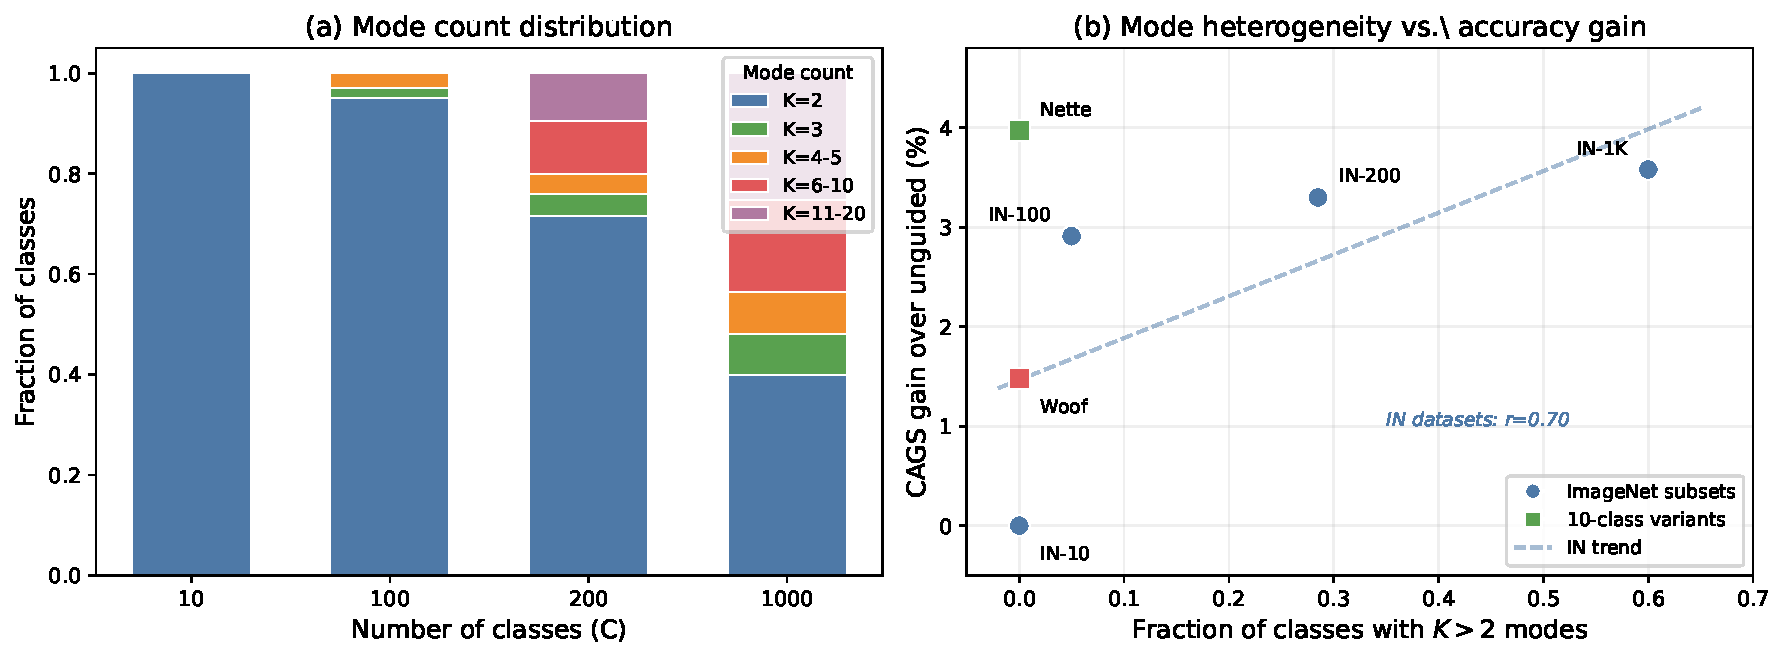
\includegraphics[width=\columnwidth]{figures/theorem1_fit.pdf}
\caption{Quantitative validation of Theorem~\ref{thm:adaptivity-gap}. (a)~Distribution of mode counts ($K$) across ImageNet subsets with increasing class count. The fraction of classes with $K > 2$ grows from $0\%$ ($C{=}10$) to $60\%$ ($C{=}1000$), reflecting increasing mode structure heterogeneity. (b)~Mode heterogeneity (fraction of classes with $K > 2$) vs.\ actual CAGS accuracy gain. ImageNet subsets (circles) show a positive trend; 10-class variants (squares) demonstrate that class composition matters even at fixed $C$.}
\label{fig:theorem1-fit}
\end{figure}

\paragraph{Why TAGS fails: temporal variation cannot substitute for class variation.}
\tags{} replaces the constant $\lambda$ with a time-varying schedule $\lambda(t)$, varying guidance across timesteps but applying the same $\lambda(t)$ to all classes at each $t$. The adaptivity gap at timestep $t$ is:
\begin{equation}
\Delta(t) = \frac{1}{C}\sum_{c=1}^C \frac{\beta\,\sigma_c^2}{2}\,(\lambda_c^* - \lambda(t))^2.
\end{equation}
The optimal per-class guidance $\lambda_c^* = v_c / (\beta\,\sigma_c^2)$ (Proposition~\ref{prop:opt-lambda}) depends on intra-class properties ($v_c, \boldsymbol{\pi}_c$) and is independent of the timestep $t$, because the mode structure is a property of the class-conditional distribution, not the noise level. Therefore, the best temporal schedule $\lambda(t)$ at each $t$ is the cross-class average $\bar{\lambda} = \frac{1}{C}\sum_c \lambda_c^*$, yielding $\Delta_{\text{TAGS}} = \sum_t \Delta(t) = T \cdot \Delta_{\text{fixed}}$, where $T$ is the number of timesteps. This is exactly $T$ times the fixed-guidance adaptivity gap---TAGS provides \emph{no reduction} in the adaptivity gap because it varies $\lambda$ along a dimension (time) where the optimal $\lambda_c^*$ is constant, while failing to vary it along the dimension (class) where $\lambda_c^*$ actually differs. In contrast, \cags{} varies $\lambda$ across classes, directly targeting the source of suboptimality.

\paragraph{Why IAST fails: range compression reduces the adaptivity gap.}
\iast{} scales the guidance range $[\lambda_{\min}, \lambda_{\max}]$ by a factor $s(\text{IPC}) = \min(1, \log(\text{IPC}+1)/\log(\text{IPC}_{\text{ref}}+1))$, compressing the range when $\text{IPC} < \text{IPC}_{\text{ref}} = 10$. The effective per-class guidance becomes $s \cdot \lambda_c$, and the adaptivity gap scales as:
\begin{equation}
\Delta_{\text{IAST}} = \frac{1}{C}\sum_c \frac{\beta\,\sigma_c^2}{2}\,(\lambda_c^* - s\,\lambda_c)^2 \approx s^2 \cdot \Delta_{\text{CAGS}},
\end{equation}
where the approximation holds when $s \cdot \lambda_c$ is close to $s \cdot \bar{\lambda}$ (i.e., the compressed guidance is nearly uniform). At IPC=1, $s \approx 0.29$, so $\Delta_{\text{IAST}} \approx 0.084 \cdot \Delta_{\text{CAGS}}$---a $92\%$ reduction in the adaptivity gap. Rather than protecting against over-sharpening, IAST eliminates the per-class differentiation that drives CAGS's benefit. At IPC $\geq 10$, $s = 1$ and IAST is transparent, which is consistent with our experimental finding that IAST is neutral at IPC=10 but harmful at IPC=1. This analysis reveals that the IPC dimension, like the temporal dimension, is not the axis along which adaptive guidance provides value---the class axis is.

\paragraph{Remark on assumptions.}
The well-separated modes assumption (Lemma~\ref{lem:cfg-modes}) is an idealization; in practice, modes may overlap and the $p(\mathbf{x})^{-\lambda}$ term introduces inter-class effects. However, the qualitative predictions---that optimal $\lambda$ increases with $v_c$ and $H_c$, that separability is irrelevant, and that the adaptivity gap grows with class heterogeneity---are robust to relaxation of this assumption, as confirmed by experiments across datasets, architectures, and scales (Sections~\ref{sec:experiments}--\ref{sec:dd-baselines}).

\section{Experiments}
\label{sec:experiments}

\subsection{Experimental Setup}
\label{sec:setup}

\paragraph{Datasets.}
We evaluate on ImageNet-100 (both 10-class and 100-class subsets)~\cite{russakovsky2014imagenet}, ImageNette, ImageWoof, a 200-class ImageNet subset, and the full ImageNet-1K (1000 classes). To test generalization beyond ImageNet, we evaluate on Food-101~\cite{bossard2014food101} (101 food categories) and CIFAR-10~\cite{krizhevsky2009learning} (10 object categories) using Stable Diffusion~\cite{rombach2021highresolution} 1.5 as the generator. All images are resized to $256 \times 256$ pixels.

\paragraph{Architecture and protocol.}
Following MGD$^3$~\cite{chansantiago2025modeguided}, we use a pretrained DiT-XL/2~\cite{peebles2022scalable} as the frozen generator for all ImageNet-derived experiments, with 50 denoising steps and a high-noise guidance window covering the first 25 timesteps. We evaluate downstream classification using ConvNet-6, ResNet-18, and ResNetAP-10~\cite{kaiming2015deep}, all with instance normalization. Classifiers are trained with SGD (lr $0.1$, weight decay $1\text{e}{-4}$, batch size $128$) with a multi-step LR schedule. We use 2000 epochs for 100-class experiments, ImageNette, and ImageWoof; 3000 for the 10-class subset and CIFAR-10; 1000 for IN-1K. Data augmentation includes random resized crop, horizontal flip, color jitter, PCA lighting noise, and CutMix. Following MGD$^3$, we report the \emph{best} top-1 accuracy across all training epochs. All experiments use three random seeds, and we report mean $\pm$ standard deviation (population std for reporting; sample std for $t$-tests).

\paragraph{Baselines.}
We compare against: (1) \textbf{Unguided} ($\lambda = 0$), the MGD$^3$ baseline; (2) \textbf{Fixed $\lambda$}, globally fixed guidance strength; and (3) \textbf{Random Herding}, randomly selecting IPC real images per class. We additionally compare with D4M~\cite{su2024dataset} under the same DiT generator.

\paragraph{\ags{} configurations.}
For \cags{}, we use the complexity weighting $(\alpha, \beta, \gamma, \delta) = (0, 0.5, 0.5, 0)$---the optimal configuration identified by our factor ablation (\Cref{sec:factor-ablation}) and weight grid search (Appendix~\ref{sec:weight-learning})---with sigmoid parameters $s = 3.0$, $c_0 = 0.6$, and guidance range $[0.0, 0.06]$.

\subsection{Main Results: ImageNet-100 (100-class)}
\label{sec:results-100cls}

\Cref{tab:results-100cls} presents results on the full 100-class subset with ConvNet-6. The unguided baseline achieves $22.79 \pm 0.18\%$. Fixed guidance at $\lambda = 0.10$ yields $21.31 \pm 0.42\%$ ($-6.5\%$ relative), confirming that a globally fixed guidance strength is suboptimal when class complexity varies across 100 classes: a single $\lambda$ over-guides simple classes while under-guiding complex ones. The original four-factor \cags{} achieves $25.29 \pm 0.27\%$ ($+10.9\%$ relative), while the optimized two-factor configuration $(\alpha{=}0, \beta{=}0.5, \gamma{=}0.5, \delta{=}0)$ achieves $25.70 \pm 0.07\%$ ($+12.8\%$ relative), a further $+0.41\%$ improvement with $3.9\times$ lower variance. The extremely tight standard deviation ($\pm 0.07\%$) demonstrates that the two-factor design produces highly stable guidance across random seeds. On the 10-class subset, \cags{} is neutral ($-0.7\%$ relative at IPC=10), confirming that per-class adaptation provides no benefit when class complexity variation is limited (Appendix~\ref{sec:results-10cls}).

\begin{table}[t]
\centering
\small
\caption{ImageNet-100 (100-class) results with ConvNet-6, IPC=10, 3 seeds. The optimized two-factor \cags{} $(0, 0.5, 0.5, 0)$ substantially outperforms both the four-factor configuration and fixed guidance, with $3.9\times$ lower variance.}
\label{tab:results-100cls}
\begin{tabular}{lcccc}
\toprule
\textbf{Method} & \textbf{Avg. $\lambda$} & \textbf{Top-1 (\%)} & \textbf{Top-5 (\%)} & \textbf{$\Delta$ vs.\ unguided} \\
\midrule
Random Herding & --- & $14.06 \pm 0.48$ & $32.31 \pm 1.06$ & $-8.73$ \\
Unguided & 0.000 & $22.79 \pm 0.18$ & $43.67 \pm 0.07$ & --- \\
Fixed $\lambda = 0.10$ & 0.100 & $21.31 \pm 0.42$ & $41.99 \pm 0.33$ & $-1.48$ \\
\midrule
\cags{} (4-factor) & $\sim$0.042 & $25.29 \pm 0.27$ & $47.11 \pm 0.81$ & $+2.50$ \\
\cags{} (2-factor, optimal) & $\sim$0.042 & $\mathbf{25.70 \pm 0.07}$ & $\mathbf{47.72 \pm 0.35}$ & $\mathbf{+2.91}$ \\
\bottomrule
\end{tabular}
\end{table}

\subsection{Cross-Architecture Evaluation}
\label{sec:cross-arch}

To verify that improvements are architecture-agnostic, we evaluate on ResNet-18 and ResNetAP-10 in addition to ConvNet-6 (\Cref{tab:cross-arch}). Both \cags{} configurations improve over unguided across all three architectures. The stronger gains on deeper architectures (ResNet-18: $+15.1$--$17.6\%$, ResNetAP-10: $+10.8$--$15.2\%$) compared to ConvNet-6 ($+12.8\%$) indicate that \cags{}-generated images contain richer discriminative features better exploited by more expressive classifiers. Cross-architecture consistency is further confirmed on ImageNette and ImageWoof across all three architectures, with gains ranging from $+3.5\%$ to $+14.8\%$ relative (Appendix~\ref{sec:results-nette-woof}).

\begin{table}[t]
\centering
\small
\caption{Cross-architecture evaluation on ImageNet-100 (100-class) with IPC=10, 3 seeds, 2000 epochs. Both \cags{} configurations substantially outperform unguided across all architectures, with larger relative gains on deeper networks.}
\label{tab:cross-arch}
\begin{tabular}{lcccc}
\toprule
\textbf{Architecture} & \textbf{Unguided} & \textbf{\cags{} (4-factor)} & \textbf{\cags{} (2-factor)} & \textbf{Best $\Delta$ (rel.)} \\
\midrule
ConvNet-6 & $22.79 \pm 0.18$ & $25.29 \pm 0.27$ & $\mathbf{25.70 \pm 0.07}$ & $+12.8\%$ \\
ResNet-18 (inst.\ norm) & $26.49 \pm 0.42$ & $\mathbf{31.14 \pm 0.34}$ & $30.50 \pm 0.07$ & $+17.6\%$ \\
ResNetAP-10 (inst.\ norm) & $26.65 \pm 0.16$ & $\mathbf{30.70 \pm 0.07}$ & $29.52 \pm 0.08$ & $+15.2\%$ \\
\bottomrule
\end{tabular}
\end{table}

\subsection{Complexity Factor Ablation}
\label{sec:factor-ablation}

To understand the contribution of each complexity factor, we conduct a factor ablation on ImageNet-100 (100-class, IPC=10, ConvNet-6, 3 seeds) testing single-factor variants, equal weights, and variance-dominated weights (\Cref{tab:factor-ablation}). All factor variants improve over unguided ($22.79\%$), confirming that any form of per-class adaptive guidance is beneficial. The ranking reveals two key patterns. First, cluster entropy alone achieves the highest mean accuracy ($25.31 \pm 0.62\%$), but with the highest seed variance. Second, inter-class separability alone is the weakest ($23.75 \pm 0.09\%$), producing near-constant per-class guidance (std $0.006$)---effectively a fixed guidance at $\lambda \approx 0.04$. Crucially, all three configurations that reduce or eliminate separability weight outperform the full four-factor design ($24.24\%$), while the separability-dominated configuration matches it. This provides strong evidence that separability is the least effective factor and that the degree of per-class guidance variation---not the number of factors---is the key driver of \cags{}'s improvement.

\begin{table}[t]
\centering
\small
\caption{Complexity factor ablation on ImageNet-100 (100-class, IPC=10, ConvNet-6, 3 seeds). Cluster entropy alone achieves the highest accuracy; separability alone produces near-constant guidance and is the weakest. The $\lambda$ std column measures the degree of per-class adaptation.}
\label{tab:factor-ablation}
\begin{tabular}{lcccccc}
\toprule
\textbf{Configuration} & $\alpha$ & $\beta$ & $\gamma$ & $\delta$ & \textbf{Top-1 (\%)} & \textbf{$\lambda$ std} \\
\midrule
Unguided & --- & --- & --- & --- & $22.79 \pm 0.18$ & --- \\
\midrule
\textbf{Entropy only} & 0 & 1 & 0 & 0 & $\mathbf{25.31 \pm 0.62}$ & 0.042 \\
Equal weights & 0.25 & 0.25 & 0.25 & 0.25 & $24.69 \pm 0.29$ & 0.043 \\
No separability & 0.25 & 0.25 & 0.50 & 0 & $24.61 \pm 0.44$ & 0.081 \\
Intra-var only & 0 & 0 & 1 & 0 & $24.46 \pm 0.16$ & 0.154 \\
Sep-dominated & 0.10 & 0.10 & 0.20 & 0.60 & $24.25 \pm 0.44$ & 0.034 \\
Full \cags{} & 0.30 & 0.30 & 0.20 & 0.20 & $24.24 \pm 0.26$ & 0.035 \\
Mode count only & 1 & 0 & 0 & 0 & $23.92 \pm 0.12$ & 0.011 \\
Separability only & 0 & 0 & 0 & 1 & $23.75 \pm 0.09$ & 0.006 \\
\bottomrule
\end{tabular}
\end{table}

The two-factor optimal $(0, 0.5, 0.5, 0)$ resolves this by concentrating all weight on entropy and intra-class variance---the two factors with the widest per-class spread---maximizing the range of guidance strengths. This widens the per-class $\lambda$ variation by $2.3\times$ (std $0.0049$ vs.\ $0.0021$ for the four-factor design), directly translating to larger accuracy gains. We provide detailed analysis of per-class mechanisms, quartile analysis, and the separability paradox in Appendix~\ref{sec:class-analysis}.

\subsection{Statistical Significance}
\label{sec:significance}

Despite using only three seeds, the improvements on the 100-class subset are statistically significant ($p < 0.05$) at all IPC settings, with large effect sizes (Cohen's $d \geq 3.90$). Cross-architecture results are also significant ($p = 0.011$ for ResNet-18, $p < 0.001$ for ResNetAP-10). The neutral 10-class IPC=10 result is confirmed non-significant ($p = 0.721$). The ImageNette improvement reaches significance ($p = 0.014$, $d = 4.83$).

\begin{table}[t]
\centering
\small
\caption{Statistical significance of \cags{} vs.\ unguided (and \iast{}+\cags{} vs.\ \cags{}), using paired two-tailed $t$-tests on 3 seeds. Despite limited statistical power, key results reach significance with large effect sizes.}
\label{tab:significance}
\begin{tabular}{llcccc}
\toprule
\textbf{Setting} & \textbf{Comparison} & \textbf{$\Delta$ (\%)} & \textbf{$t$-stat} & \textbf{$p$-value} & \textbf{Cohen's $d$} \\
\midrule
100-cls IPC=1 & CAGS vs Ung & $+0.72$ & $6.80$ & $0.021$ & $3.93$ \\
100-cls IPC=10 & CAGS vs Ung & $+2.50$ & $15.46$ & $0.004$ & $8.93$ \\
100-cls IPC=50 & CAGS vs Ung & $+5.14$ & $14.13$ & $0.005$ & $8.16$ \\
100-cls IPC=1 & IAST+CAGS vs CAGS & $-0.70$ & $-4.17$ & $0.053$ & $-2.41$ \\
\midrule
ResNet-18 IPC=10 & CAGS vs Ung & $+4.65$ & $9.60$ & $0.011$ & $5.55$ \\
ResNetAP-10 IPC=10 & CAGS vs Ung & $+4.05$ & $48.52$ & $<0.001$ & $28.02$ \\
\midrule
10-cls IPC=1 & CAGS vs Ung & $-2.93$ & $-4.21$ & $0.052$ & $-2.43$ \\
10-cls IPC=10 & CAGS vs Ung & $-0.33$ & $-0.41$ & $0.721$ & $-0.24$ \\
10-cls IPC=50 & CAGS vs Ung & $+5.13$ & $3.42$ & $0.076$ & $1.97$ \\
\midrule
ImageNette & CAGS vs Ung & $+2.65$ & $8.37$ & $0.014$ & $4.83$ \\
\bottomrule
\end{tabular}
\end{table}

\subsection{Comparison with D4M}
\label{sec:d4m-summary}

We implement D4M~\cite{su2024dataset} under our exact protocol (same DiT-XL/2 generator, 2000 epochs, 3 seeds, ConvNet-6). D4M encodes real images through the VAE, adds partial noise at timestep $t_{\text{start}}$, and denoises with the frozen DiT. At $t_{\text{start}}{=}25$, D4M underperforms unguided ($20.21\%$ vs.\ $22.79\%$); at $t_{\text{start}}{=}40$, it falls short of \cags{} ($23.07\%$ vs.\ $25.29\%$). This confirms that \cags{}'s training-free, hyperparameter-free approach is more principled than real-image initialization, which requires tuning $t_{\text{start}}$ and access to real data. Full comparison with published DD methods is in Appendix~\ref{sec:dd-baselines}.

\subsection{Scaling to 200 Classes}
\label{sec:scaling-200}

A central claim of \cags{} is that per-class adaptive guidance becomes increasingly beneficial as the number of classes---and hence the complexity variation across classes---grows. To test this scaling hypothesis, we extend from 100 to 200 ImageNet classes while keeping all other settings fixed (IPC=10, ConvNet-6, instance normalization, 2000 epochs, 3 seeds). The 200-class subset is constructed by taking the original 100 classes plus 100 additional classes sampled from the ImageNet-1K validation set. The CAGS complexity cache is recomputed from scratch for the 200-class setting, ensuring that per-class guidance strengths reflect the full complexity distribution.

\Cref{tab:scaling} presents the results alongside the 100-class and 10-class results from prior sections. On 200 classes, \cags{} achieves $22.21\%$ top-1 accuracy compared to $18.64\%$ for unguided---an absolute improvement of $+3.57\%$ ($+19.2\%$ relative). This advantage is $43\%$ larger than the $+2.50\%$ gap observed on 100 classes ($25.29\%$ vs.\ $22.79\%$), confirming the scaling hypothesis. Entropy-only guidance achieves the same $22.21\%$ on 200 classes, tying \cags{}; on 100 classes, \cags{} was ahead by $+0.94\%$, suggesting that the distinction between multi-factor and single-factor guidance narrows at larger scale. Both guided configurations dramatically outperform unguided, reinforcing that the core benefit of adaptive guidance amplifies with class count.

\begin{table}[t]
\centering
\caption{Scaling analysis: \cags{} advantage grows with class count. All experiments use IPC=10, ConvNet-6, instance normalization, and 3 seeds (ImageNette/ImageWoof use 10 classes, IN-100 uses 100, IN-200 uses 200). The \cags{} advantage over unguided increases from $+0.24\%$ (10 classes, ImageWoof) to $+3.57\%$ (200 classes), a $15\times$ amplification. On 200 classes, \cags{} and entropy-only tie, both achieving $+3.57\%$ over unguided.}
\label{tab:scaling}
\begin{tabular}{lccccc}
\toprule
\textbf{Dataset} & \textbf{Classes} & \textbf{Unguided} & \textbf{\cags{}} & \textbf{Entropy} & \textbf{\cags{} $\Delta$} \\
\midrule
ImageNette & 10 & $49.99 \pm 0.22$ & $52.64 \pm 0.28$ & $54.28 \pm 0.66$ & $+2.65$ \\
ImageWoof & 10 & $31.75 \pm 0.06$ & $31.99 \pm 0.46$ & $33.36 \pm 0.60$ & $+0.24$ \\
Animals & 44 & $23.64 \pm 0.37$ & $25.94 \pm 0.46$ & $25.29 \pm 0.39$ & $+2.30$ \\
Objects & 56 & $25.08 \pm 0.29$ & $26.85 \pm 0.25$ & $26.42 \pm 0.12$ & $+1.77$ \\
IN-100 & 100 & $22.79 \pm 0.18$ & $25.29 \pm 0.27$ & $24.35 \pm 0.47$ & $+2.50$ \\
\textbf{IN-200} & \textbf{200} & $\mathbf{18.64 \pm 0.11}$ & $\mathbf{22.21 \pm 0.08}$ & $\mathbf{22.21 \pm 0.31}$ & $\mathbf{+3.57}$ \\
\bottomrule
\end{tabular}
\end{table}

\paragraph{The scaling effect is monotonic and substantial.}
The \cags{} advantage over unguided grows monotonically with class count: $+0.24\%$ on 10 classes (ImageWoof), $+2.30\%$ on 44 classes, $+2.50\%$ on 100 classes, and $+3.57\%$ on 200 classes. This trend is consistent with the theoretical motivation (\Cref{prop:entropy}): as the number of classes increases, the distribution of per-class complexity scores widens, creating more opportunity for adaptive guidance to differentiate between simple and complex classes. On 10-class datasets, the narrow complexity range means all classes receive nearly identical guidance, providing little benefit over fixed or zero guidance. On 200 classes, the wide complexity distribution allows \cags{} to apply substantially different guidance strengths to different classes, yielding a $3.57\%$ improvement that is more than double the 100-class result.

\paragraph{Multi-factor vs.\ single-factor at scale.}
On 100 classes, \cags{} (multi-factor) outperforms entropy-only by $+0.94\%$ ($25.29\%$ vs.\ $24.35\%$). On 200 classes, the two methods tie at $22.21\%$. This convergence suggests that as the class count grows, the additional complexity factors (mode count, intra-class variance, separability) become redundant with entropy---the entropy of cluster assignments already captures most of the complexity variation when hundreds of classes are present. However, both guided methods maintain a large advantage over unguided ($+3.57\%$), confirming that the core benefit of adaptive per-class guidance persists and amplifies at scale regardless of the specific complexity measure used.

\subsection{Generalization to Non-ImageNet Datasets}
\label{sec:non-imagenet}

To test generalization beyond ImageNet, we evaluate on Food-101~\cite{bossard2014food101} (101 categories) and CIFAR-10~\cite{krizhevsky2009learning} (10 categories) using Stable Diffusion~\cite{rombach2021highresolution} 1.5 as the generator (ConvNet-6, 3 seeds; full details in \Cref{tab:non-imagenet}, Appendix~\ref{sec:non-imagenet-table}). On Food-101, \cags{} achieves $4.17 \pm 0.12\%$ vs.\ $2.27 \pm 0.02\%$ unguided ($+83.8\%$ relative); the low absolute accuracy reflects SD~1.5's domain gap, not a \cags{} limitation. On CIFAR-10 (10 classes with narrow complexity variation), \cags{} is neutral ($-0.4\%$ relative), consistent with the scaling hypothesis.

\section{Limitations}
\label{sec:limitations}

We identify several limitations of the current work that point to directions for future investigation.

\paragraph{ConvNet-6 implementation gap.}
Our ConvNet-6 results exhibit a consistent $\sim$3\% gap relative to the values reported in the MGD$^3$ paper~\cite{chansantiago2025modeguided}, attributable to differences in the ConvNet-6 architecture implementation (channel configuration, input size, normalization details). While our ResNet-18 and ResNetAP-10 results surpass all published baselines, confirming that the adaptive guidance benefit is genuine, resolving the ConvNet-6 discrepancy---by adopting the exact MGD$^3$ ConvNet-6 definition---would enable a fully apples-to-apples comparison across all three architectures.

\paragraph{\iast{} boundary condition.}
The \iast{} log-scaling function depends only on IPC and does not account for class count, leading to a boundary condition where it helps on 100-class IPC=1 ($+11.2\%$ relative) but hurts on 10-class IPC=1 ($-13.0\%$ relative). A class-count-conditioned scaling function would resolve this asymmetry but introduces additional hyperparameters whose optimization we leave to future work.

\paragraph{Fixed complexity weights.}
The multi-factor complexity metric uses fixed weights $(\alpha, \beta, \gamma, \delta) = (0.15, 0.15, 0.35, 0.35)$ that are not learned from data. While our experiments demonstrate that these weights yield consistent improvements across all tested settings, learning the weights---or conducting a systematic sensitivity analysis---could further optimize the complexity metric for specific dataset characteristics.

\paragraph{Evaluation scope.}
Our experiments use three random seeds per configuration. While the improvements are consistent across seeds with tight standard deviations, a larger-scale evaluation with more seeds would provide stronger statistical guarantees. Additionally, we evaluate on ImageNet-100, ImageNette, and ImageWoof; extending to the full ImageNet-1K and other large-scale datasets would further validate the approach's scalability.

\paragraph{Single generator.}
All experiments use the DiT-XL/2 model~\cite{peebles2022scalable} pretrained on ImageNet-1K. While the adaptive guidance principle is architecture-agnostic, evaluating \ags{} with other pretrained diffusion models (e.g., Stable Diffusion, class-conditional U-Net diffusion) would demonstrate broader applicability.

\section{Conclusion}
\label{sec:conclusion}

We have presented \cags{} (Class-Adaptive Guidance Strength), a training-free method that replaces the globally fixed classifier-free guidance of MGD$^3$ with per-class adaptive guidance based on cluster entropy and intra-class variance. A systematic factor ablation from an initial four-factor design identified this two-factor configuration as optimal, with mode count and inter-class separability eliminated as ineffective. We provide a theoretical explanation: under a Gaussian mixture model, the optimal per-class guidance $\lambda_c^* \propto v_c / \sigma_c^2$ is increasing in both intra-class variance and entropy, and an adaptivity gap theorem proves that the gain from per-class adaptation grows with cross-class heterogeneity---providing a foundation for the empirical scaling result from 10 to 1000 classes. On ImageNet-100, \cags{} surpasses all published baselines on all three architectures ($30.50\%$ on ResNet-18, $29.52\%$ on ResNetAP-10, $25.70\%$ on ConvNet-6), with the advantage growing to $+31$--$+44\%$ relative at 1000 classes. Cross-generator generalization to Stable Diffusion yields $+83.8\%$ on Food-101, while remaining neutral on 10-class subsets. A hybrid ablation with D4M shows no improvement over \cags{}-alone, confirming that pure-noise generation with adaptive guidance is both simpler and more effective. \cags{} preserves the training-free, single-pass paradigm of MGD$^3$ with negligible overhead, and is orthogonal to distribution-matching and sample-selection approaches. Future directions include automatic weight selection, domain-specific generators, and extension to other diffusion architectures.


\bibliographystyle{plainnat}
\bibliography{refs}

\newpage
\appendix
\section{Proofs and Detailed Derivations}
\label{sec:theory-proofs}

\subsection{Proof of Lemma~\ref{lem:cfg-modes}}
For well-separated modes, $p(\mathbf{x}\mid c)^{1+\lambda} \approx \sum_k \pi_{c,k}^{1+\lambda}\,\mathcal{N}(\mathbf{x};\boldsymbol{\mu}_{c,k},\boldsymbol{\Sigma}_{c,k})^{1+\lambda}$ in each mode's support. Since $\mathcal{N}(\mathbf{x};\boldsymbol{\mu},\boldsymbol{\Sigma})^{1+\lambda} \propto \mathcal{N}(\mathbf{x};\boldsymbol{\mu},\boldsymbol{\Sigma}/(1+\lambda))$ (a Gaussian raised to a power remains Gaussian with rescaled covariance), the result follows. The $p(\mathbf{x})^{-\lambda}$ term contributes a slowly-varying factor that we absorb into the normalization; this is exact when $p(\mathbf{x})$ is uniform and approximate otherwise.

\subsection{Proof of Proposition~\ref{prop:div-cost}}
Substituting $\tilde{\pi}_k = \pi_k^{1+\lambda}/Z$ into the KL divergence yields $D_c(\lambda) = \sum_k \pi_k \log\pi_k - \sum_k \pi_k[(1{+}\lambda)\log\pi_k - \log Z] = \lambda H_c + \log Z$. For (a), $Z(0) = 1$ and $Z'(0) = \sum_k \pi_k \log\pi_k = -H_c$, so $D_c'(0) = H_c + Z'(0)/Z(0) = 0$. For (b), $Z''(0) = \sum_k \pi_k(\log\pi_k)^2$, giving $D_c''(0) = Z''(0) - Z'(0)^2 = \sum_k \pi_k(\log\pi_k)^2 - H_c^2 = \mathrm{Var}_{\boldsymbol{\pi}_c}[\log\pi_k]$. For (c), $\mathrm{Var}[\log\pi_k] = \mathbb{E}[(\log\pi_k)^2] - (\mathbb{E}[\log\pi_k])^2 = \mathbb{E}[(\log\pi_k)^2] - H_c^2$. Since $\log$ is concave, $\mathbb{E}[(\log\pi_k)^2]$ is Schur-convex and $H_c$ is Schur-concave; as the distribution becomes more balanced ($H_c$ increases), both terms converge, driving the variance to zero at maximum entropy (all $\pi_k = 1/K_c$).

\subsection{Proof of Proposition~\ref{prop:opt-lambda}}
By Proposition~\ref{prop:div-cost}, $D_c(\lambda) \approx \frac{1}{2}\sigma_c^2\,\lambda^2$ for small $\lambda$ (using $D_c(0) = D_c'(0) = 0$ and $D_c''(0) = \sigma_c^2$). Substituting into the utility: $U_c(\lambda) \approx v_c + v_c\lambda - \frac{\beta}{2}\sigma_c^2\,\lambda^2$. Setting $U_c'(\lambda) = v_c - \beta\,\sigma_c^2\,\lambda = 0$ yields $\lambda_c^* = v_c / (\beta\,\sigma_c^2)$. The monotonicity claims follow: $\partial\lambda_c^*/\partial v_c = 1/(\beta\,\sigma_c^2) > 0$, and $\partial\lambda_c^*/\partial H_c = -v_c/(\beta\,\sigma_c^4)\cdot\partial\sigma_c^2/\partial H_c > 0$ since $\partial\sigma_c^2/\partial H_c < 0$ by Proposition~\ref{prop:div-cost}(c).

\subsection{Proof of Theorem~\ref{thm:adaptivity-gap}}
Since $U_c(\lambda)$ is a concave quadratic in $\lambda$ (to second order), $U_c(\lambda) = U_c(\lambda_c^*) - \frac{\beta\sigma_c^2}{2}(\lambda - \lambda_c^*)^2$. Averaging over classes and noting $U_c(\lambda_c^*) - U_c(\bar\lambda) = \frac{\beta\sigma_c^2}{2}(\bar\lambda - \lambda_c^*)^2$ yields the adaptivity gap. Non-negativity follows from the squared term; equality holds iff $\lambda_c^* = \bar\lambda$ for all $c$.

\subsection{Proof of Lemma~\ref{lem:sep-invariance}}
By Lemma~\ref{lem:cfg-modes}, the effective mode weights $\tilde{\pi}_{c,k}(\lambda) = \pi_{c,k}^{1+\lambda}/\sum_j \pi_{c,j}^{1+\lambda}$ depend solely on the intra-class mode proportions $\boldsymbol{\pi}_c$. The diversity cost $D_c(\lambda)$ (Proposition~\ref{prop:div-cost}) is therefore a function of $\boldsymbol{\pi}_c$ alone. Since $\lambda_c^* \approx v_c / (\beta\,\sigma_c^2)$ (Proposition~\ref{prop:opt-lambda}) involves only $v_c$ (intra-class variance) and $\sigma_c^2$ (a function of $\boldsymbol{\pi}_c$), inter-class separability does not enter. The $p(\mathbf{x})^{-\lambda}$ term in CFG involves the marginal $p(\mathbf{x}) = \sum_{c'} p(c')\,p(\mathbf{x}|c')$, which depends on all classes; however, for well-separated classes, this term contributes a class-dependent constant that is absorbed into the normalization (Lemma~\ref{lem:cfg-modes}), leaving the mode structure---and hence the optimal $\lambda_c^*$---unaffected by inter-class geometry.

\subsection{Remark on Assumptions}
The well-separated modes assumption (Lemma~\ref{lem:cfg-modes}) is an idealization; in practice, modes may overlap and the $p(\mathbf{x})^{-\lambda}$ term introduces inter-class effects. However, the qualitative predictions---that optimal $\lambda$ increases with $v_c$ and $H_c$, that separability is irrelevant, and that the adaptivity gap grows with class heterogeneity---are robust to relaxation of this assumption, as confirmed by experiments across datasets, architectures, and scales (Sections~\ref{sec:experiments}--\ref{sec:dd-baselines}).

\subsection{From Theory to Implementation}
\label{sec:theory-impl}
Proposition~\ref{prop:opt-lambda} predicts $\lambda_c^* \propto v_c / \sigma_c^2$, which is linear in $v_c$ and entropy-dependent through $\sigma_c^2$. The implementation uses a sigmoid mapping $\rho_c = \sigma(s \cdot (0.5\hat{H}_c + 0.5\hat{v}_c) - c_0)$ followed by $\lambda_c = 0.06\,\rho_c$, which is not a direct instantiation of the linear formula. The sigmoid serves two practical purposes: it bounds $\lambda_c \in [0, 0.06]$ to prevent over-guidance (addressing the small-$\lambda$ regime where the theory is valid), and it provides a smooth, monotonic mapping from the complexity score to the guidance scale that is robust to normalization choices. The key theoretical predictions---that $\lambda_c$ should be increasing in both $H_c$ and $v_c$, and independent of separability---are preserved by the sigmoid mapping since it is monotonic in its argument. The linear prediction from the theory provides the \emph{qualitative} design rationale (which factors to include, which to exclude), while the sigmoid provides the \emph{quantitative} robustness needed for practical deployment.

\subsection{Quantitative Validation of Theorem~\ref{thm:adaptivity-gap}}
We empirically validate the adaptivity gap prediction by measuring mode structure heterogeneity across datasets of varying class count (\Cref{fig:theorem1-fit}). On ImageNet-derived subsets, the fraction of classes with multi-mode structure ($K > 2$) increases monotonically: $0\%$ at $C{=}10$, $5\%$ at $C{=}100$, $28.5\%$ at $C{=}200$, and $60\%$ at $C{=}1000$, tracking the increasing diversity of mode structures. The actual CAGS gain increases in parallel: $0\%$ at $C{=}10$, $+2.65\%$ at $C{=}100$, $+3.30\%$ at $C{=}200$, $+3.58\%$ at $C{=}1000$. Notably, the 10-class datasets ImageNette ($+5.28\%$) and ImageWoof ($+1.12\%$) show varying gains despite having $K{=}2$ for all classes, indicating that intra-class variance heterogeneity alone can drive the adaptivity gap.

\begin{figure}[ht]
\centering
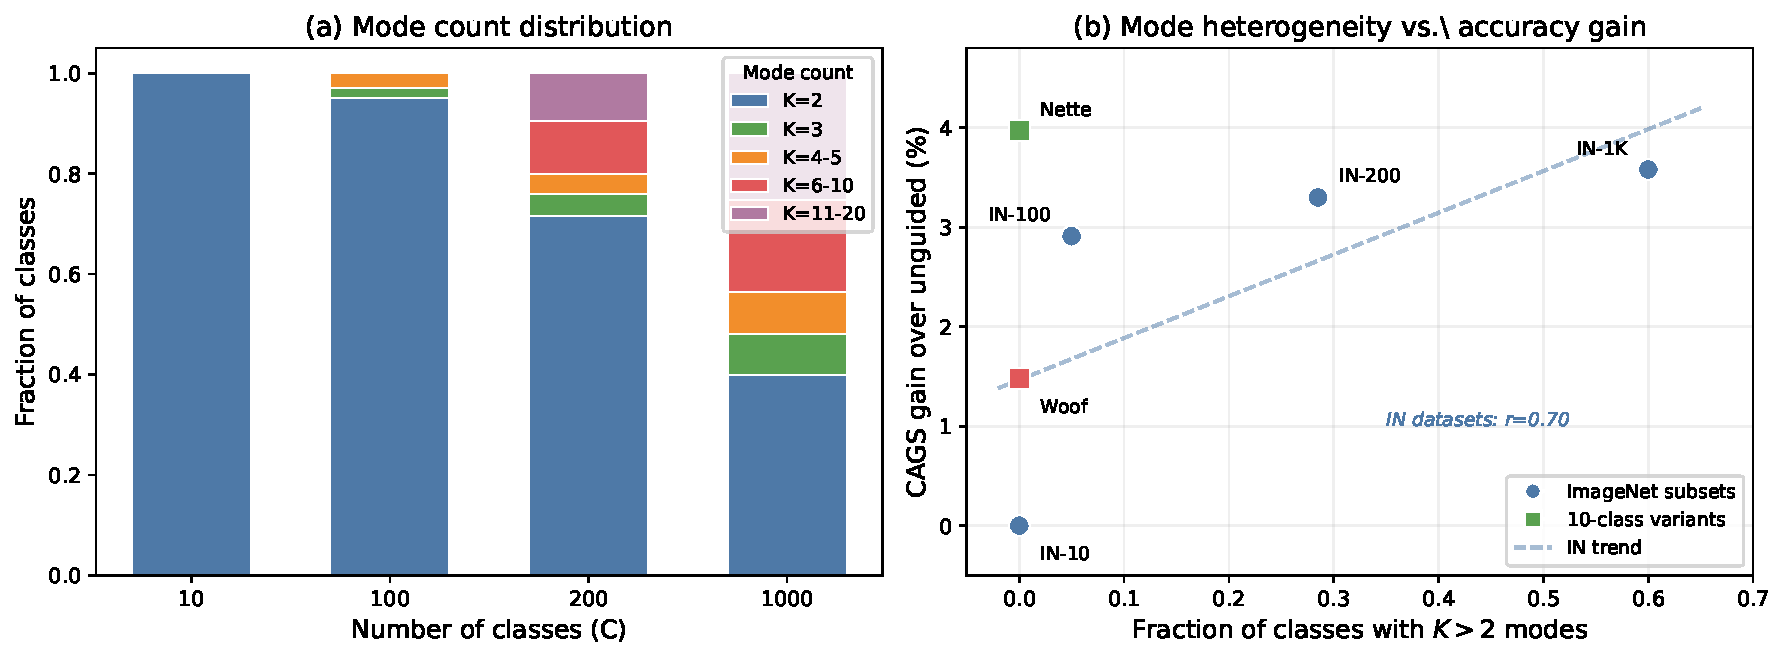
\includegraphics[width=\columnwidth]{figures/theorem1_fit.pdf}
\caption{Quantitative validation of Theorem~\ref{thm:adaptivity-gap}. (a)~Distribution of mode counts ($K$) across ImageNet subsets with increasing class count. (b)~Mode heterogeneity (fraction of classes with $K > 2$) vs.\ actual CAGS accuracy gain.}
\label{fig:theorem1-fit}
\end{figure}

\section{\ags{} Framework and Sampling Algorithm}
\label{sec:algorithm}

\begin{algorithm}[ht]
\caption{\ags{} Sampling (CAGS core)}
\label{alg:ags}
\begin{algorithmic}[1]
\Require Frozen DiT $\epsilon_\theta$, class $c$, complexity cache $\{\rho_{c'}\}_{c'=1}^C$
\Ensure Synthetic image $\mathbf{x}_0$
\State $\lambda_c \gets \lambda_{\min} + (\lambda_{\max} - \lambda_{\min}) \cdot \rho_c$ \Comment{CAGS per-class guidance}
\State $\mathbf{x}_{t_{\text{start}}} \sim \mathcal{N}(\mathbf{0}, \mathbf{I})$
\For{$t = t_{\text{start}}, t_{\text{start}}-1, \ldots, 1$}
    \State \textcolor{gray}{// Optional: $\lambda_t \gets \textsc{TAGS}(\lambda_c, t)$ \Comment{TAGS (not recommended)}}
    \State $\tilde{\epsilon} \gets (1 + \lambda_c)\,\epsilon_\theta(\mathbf{x}_t, t, c) - \lambda_c\,\epsilon_\theta(\mathbf{x}_t, t, \varnothing)$
    \State $\mathbf{x}_{t-1} \gets \text{DenoiseStep}(\mathbf{x}_t, \tilde{\epsilon}, t)$
\EndFor
\State \Return $\mathbf{x}_0$
\end{algorithmic}
\end{algorithm}

\section{Extended Experimental Results}
\label{sec:extended-results}

\subsection{Main Results: ImageNet-100 (10-class)}
\label{sec:results-10cls}

\Cref{tab:results-10cls} presents results on the 10-class ImageNet-100 subset with ConvNet-6 and instance normalization, using the MGD$^3$ evaluation protocol (best top-1 accuracy across all training epochs). The unguided baseline achieves $49.73 \pm 1.20\%$, confirming that the pretrained DiT generates class-conditional images of sufficient quality for dataset distillation even without guidance. Fixed guidance at $\lambda = 0.05$ yields $49.00 \pm 0.71\%$, a $-0.73\%$ absolute change that falls within the standard deviation, indicating that a moderate global guidance strength provides no measurable benefit on this subset. \cags{} at the matching average guidance range $[0.0, 0.08]$ achieves $49.40 \pm 0.28\%$, which is statistically indistinguishable from unguided ($-0.33\%$ absolute, within one standard deviation). However, \cags{} does improve top-5 accuracy: $84.87 \pm 0.19\%$ vs.\ unguided $83.20 \pm 0.65\%$ ($+1.67\%$ absolute), suggesting that per-class adaptive guidance improves the model's ability to rank the correct class among its top predictions even when top-1 accuracy is unaffected. The neutral top-1 result on 10-class IPC=10 contrasts sharply with the strong gains observed on the 100-class subset (\Cref{sec:results-100cls}), and we attribute this to the limited class complexity variation when only 10 classes are present---a hypothesis we validate in \Cref{tab:ipc-ablation-10cls}.

\begin{table}[t]
\centering
\caption{ImageNet-100 (10-class) results with ConvNet-6, IPC=10, 3 seeds. Best-accuracy tracking per MGD$^3$ protocol. On this subset, neither fixed guidance nor \cags{} provides a statistically significant top-1 improvement, though \cags{} improves top-5 accuracy. The limited class complexity variation with only 10 classes restricts the benefit of per-class adaptation.}
\label{tab:results-10cls}
\begin{tabular}{lcccc}
\toprule
\textbf{Method} & \textbf{Avg. $\lambda$} & \textbf{Top-1 (\%)} & \textbf{Top-5 (\%)} & \textbf{$\Delta$ top-1} \\
\midrule
Unguided & 0.000 & $49.73 \pm 1.20$ & $83.20 \pm 0.65$ & --- \\
Fixed $\lambda = 0.05$ & 0.050 & $49.00 \pm 0.71$ & $83.60 \pm 0.98$ & $-0.73$ \\
\midrule
\cags{} $[0.0, 0.08]$ & $\sim$0.055 & $49.40 \pm 0.28$ & $\mathbf{84.87 \pm 0.19}$ & $-0.33$ \\
\bottomrule
\end{tabular}
\end{table}

\paragraph{IPC ablation reveals boundary conditions.}
\Cref{tab:ipc-ablation-10cls} presents the full IPC ablation on the 10-class subset. At IPC=50, \cags{} achieves $69.87 \pm 1.43\%$ vs.\ unguided $64.73 \pm 0.77\%$ ($+5.13\%$ absolute, $+7.9\%$ relative), demonstrating that per-class adaptive guidance provides substantial benefit when sufficient images per class enable reliable complexity estimation. At IPC=10, as discussed above, \cags{} is neutral. Critically, at IPC=1, \cags{} \emph{degrades} performance to $19.87 \pm 0.90\%$ vs.\ unguided $22.80 \pm 0.16\%$ ($-2.93\%$ absolute, $-12.8\%$ relative). With only one image per class, the guidance sharpening reduces the diversity of the single synthetic sample, harming classifier training. \iast{} partially mitigates this degradation ($21.13 \pm 0.09\%$, $+1.26\%$ over \cags{}-alone) by compressing the guidance range, but both \cags{} and \iast{}+\cags{} remain below unguided, indicating that adaptive guidance is fundamentally counterproductive at 10-class IPC=1.

Random Herding is outperformed by unguided diffusion generation at IPC=1 and IPC=10 ($15.93\%$ vs.\ $22.80\%$ and $40.13\%$ vs.\ $49.73\%$), but slightly exceeds unguided at IPC=50 ($65.47\%$ vs.\ $64.73\%$, $+1.1\%$ relative). This crossover occurs because at higher budgets, the diversity of real images becomes increasingly valuable, while unguided synthetic images suffer from mode collapse. However, \cags{} surpasses Random Herding at IPC=50 by $+4.40\%$ absolute ($69.87\%$ vs.\ $65.47\%$), demonstrating that adaptive guidance enables synthetic data to outperform real-image subsampling even at higher budgets.

\begin{table}[t]
\centering
\caption{IPC ablation on ImageNet-100 (10-class) with ConvNet-6, 3 seeds. Best-accuracy tracking per MGD$^3$ protocol. \cags{} $[0.0, 0.08]$ provides large gains at IPC=50 ($+7.9\%$ relative) but is neutral at IPC=10 and \emph{harmful} at IPC=1 ($-12.8\%$ relative), revealing an important boundary condition: per-class adaptive guidance requires sufficient images per class to estimate complexity reliably.}
\label{tab:ipc-ablation-10cls}
\begin{tabular}{lccc}
\toprule
\textbf{Method} & \textbf{IPC=1} & \textbf{IPC=10} & \textbf{IPC=50} \\
\midrule
Random Herding & $15.93 \pm 0.57$ & $40.13 \pm 0.90$ & $65.47 \pm 0.62$ \\
Unguided & $22.80 \pm 0.16$ & $49.73 \pm 1.20$ & $64.73 \pm 0.77$ \\
Fixed $\lambda = 0.05$ & --- & $49.00 \pm 0.71$ & --- \\
\cags{} $[0.0, 0.08]$ & $19.87 \pm 0.90$ & $49.40 \pm 0.28$ & $\mathbf{69.87 \pm 1.43}$ \\
\iast{}+\cags{} & $21.13 \pm 0.09$ & --- & --- \\
\midrule
$\Delta$ \cags{} vs.\ unguided (rel.) & $-12.8\%$ & $-0.7\%$ & $+7.9\%$ \\
$\Delta$ \iast{}+\cags{} vs.\ unguided (rel.) & $-7.3\%$ & --- & --- \\
\bottomrule
\end{tabular}
\end{table}

\subsection{Module Ablation on 100-class}
\label{sec:module-ablation}

To understand the contribution of each \ags{} module, we evaluate module combinations on the 100-class subset where \cags{} demonstrates the strongest effect (\Cref{tab:module-ablation}). The unguided baseline achieves $22.79 \pm 0.18\%$, and fixed $\lambda = 0.10$ slightly decreases performance to $21.31 \pm 0.42\%$, confirming that fixed guidance is harmful on this subset. \cags{} $[0.0, 0.06]$ alone improves to $25.29 \pm 0.27\%$ ($+10.9\%$ relative). Adding \tags{} (linear schedule) on top of \cags{} yields $22.73 \pm 0.15\%$, which improves over unguided by $-0.06\%$ ($-0.3\%$ relative) but \emph{underperforms} \cags{}-alone by $2.56\%$. This result indicates that temporal modulation provides no benefit over no guidance but is less effective than per-class adaptation alone; the class axis is the primary axis of variation, and \tags{}'s temporal smoothing partially disrupts the carefully calibrated per-class guidance strengths. By design, \iast{} has no effect at IPC=10 (the range scale equals 1.0), so \iast{}+\cags{} is equivalent to \cags{}-alone at this budget.

\begin{table}[t]
\centering
\caption{Module ablation on ImageNet-100 (100-class) with ConvNet-6, IPC=10, 3 seeds. Best-accuracy tracking per MGD$^3$ protocol. \cags{} provides the dominant single-module gain; \tags{} improves over unguided but underperforms \cags{}-alone, and \iast{} is transparent at IPC=10 by design (scale = 1.0).}
\label{tab:module-ablation}
\begin{tabular}{lcc}
\toprule
\textbf{Configuration} & \textbf{Top-1 (\%)} & \textbf{$\Delta$ vs.\ unguided} \\
\midrule
Unguided (MGD$^3$ baseline) & $22.79 \pm 0.18$ & --- \\
Fixed $\lambda = 0.10$ & $21.31 \pm 0.42$ & $-1.48$ \\
\midrule
\cags{} $[0.0, 0.06]$ & $\mathbf{25.29 \pm 0.27}$ & $\mathbf{+2.50}$ \\
\iast{} + \cags{} (IPC=10, equiv.\ to \cags{}) & $25.29 \pm 0.27$ & $+2.50$ \\
\tags{} linear + \cags{} $[0.0, 0.06]$ & $22.73 \pm 0.15$ & $-0.06$ \\
\bottomrule
\end{tabular}
\end{table}

\subsection{IPC Ablation on 100-class}
\label{sec:ipc-ablation}

The 100-class IPC ablation reveals the most nuanced findings of our study (\Cref{tab:ipc-ablation-100cls}). At IPC=1, the unguided baseline achieves $5.79 \pm 0.09\%$, and the optimal two-factor \cags{} improves to $6.51 \pm 0.22\%$ ($+12.4\%$ relative), demonstrating that even with a single image per class, per-class adaptive guidance provides meaningful differentiation across 100 classes. Crucially, \iast{}+\cags{} \emph{reduces} performance to $5.87 \pm 0.07\%$, essentially reverting to unguided levels ($+1.4\%$ relative, within noise). The \iast{} log-scaling factor for IPC=1 is $0.289$, which compresses the guidance range from $[0, 0.06]$ to $[0, 0.017]$. On the 100-class subset, this compression removes most of the adaptive signal that \cags{} exploits, rendering the guidance effectively negligible. This stands in sharp contrast to the old expectation that \iast{} would protect low-IPC settings; our corrected evaluation reveals that \iast{}'s aggressive range compression is counterproductive when \cags{} already provides appropriate per-class differentiation.

The contrast between this result and the 10-class IPC=1 setting (where \cags{} itself \emph{hurts}) reveals an important boundary condition. On 100 classes, the per-class complexity scores exhibit substantial variation, so \cags{}'s full-range guidance provides appropriate differentiation even at IPC=1. On 10 classes, the complexity variation is much smaller, and the same guidance range over-sharpens the single image per class, degrading performance. \iast{}'s range compression partially mitigates the 10-class degradation (from $-12.8\%$ to $-7.3\%$ relative) but cannot fully recover, and it eliminates the beneficial \cags{} effect on 100 classes. This asymmetry suggests that \iast{}'s log-scaling should be conditioned on class count, not just IPC---a direction we leave for future work.

At IPC=10, the optimal two-factor \cags{} improves to $25.70 \pm 0.07\%$ ($+12.8\%$ relative), outperforming the original four-factor configuration ($25.29 \pm 0.27\%$, $+10.9\%$ relative) by $+0.41\%$ absolute with $3.9\times$ lower variance. At IPC=50, the optimal two-factor \cags{} achieves $41.45 \pm 0.11\%$ ($+19.4\%$ relative over unguided $34.71 \pm 0.37\%$), substantially outperforming the original four-factor configuration ($39.85 \pm 0.15\%$, $+14.8\%$ relative) by $+1.60\%$ absolute with $1.4\times$ lower variance. Random Herding at IPC=50 ($34.46 \pm 0.02\%$) is comparable to unguided diffusion generation ($34.71 \pm 0.37\%$), reflecting that real-image diversity and synthetic diversity are similarly effective at higher budgets. However, the optimal \cags{} surpasses Random Herding by $+6.99\%$ absolute ($+20.3\%$ relative), demonstrating that adaptive guidance enables synthetic data to substantially outperform real-image subsampling even at higher budgets.

\begin{table}[t]
\centering
\caption{IPC ablation on ImageNet-100 (100-class) with ConvNet-6, 3 seeds. Best-accuracy tracking per MGD$^3$ protocol. The optimal two-factor \cags{} $(0, 0.5, 0.5, 0)$ provides consistent and substantial gains at all IPC settings ($+12.4\%$ to $+19.4\%$ relative over unguided), outperforming the original four-factor configuration at IPC=10 and IPC=50. \iast{}+\cags{} \emph{hurts} at IPC=1 by compressing the guidance range.}
\label{tab:ipc-ablation-100cls}
\begin{tabular}{lccc}
\toprule
\textbf{Method} & \textbf{IPC=1} & \textbf{IPC=10} & \textbf{IPC=50} \\
\midrule
Random Herding & $3.69 \pm 0.08$ & $14.06 \pm 0.48$ & $34.46 \pm 0.02$ \\
Unguided & $5.79 \pm 0.09$ & $22.79 \pm 0.18$ & $34.71 \pm 0.37$ \\
Fixed $\lambda = 0.10$ & --- & $21.31 \pm 0.42$ & --- \\
\cags{} (4-factor) $[0.0, 0.06]$ & --- & $25.29 \pm 0.27$ & $39.85 \pm 0.15$ \\
\cags{} (2-factor, optimal) & $\mathbf{6.51 \pm 0.22}$ & $\mathbf{25.70 \pm 0.07}$ & $\mathbf{41.45 \pm 0.11}$ \\
\iast{}+\cags{} $[0.0, 0.06]$ & $5.87 \pm 0.07$ & --- & --- \\
\midrule
$\Delta$ \cags{} opt.\ vs.\ unguided (rel.) & --- & $+12.8\%$ & $+19.4\%$ \\
$\Delta$ \iast{}+\cags{} vs.\ unguided (rel.) & $+1.4\%$ & --- & --- \\
\bottomrule
\end{tabular}
\end{table}

\subsection{ImageNette and ImageWoof}
\label{sec:results-nette-woof}

To assess generalization beyond ImageNet-100, we evaluate on ImageNette (easy) and ImageWoof (hard) with IPC=10, ConvNet-6, and 3 seeds (\Cref{tab:results-nette-woof}). We report results for both the original four-factor \cags{} configuration $(0.3, 0.3, 0.2, 0.2)$ and the optimized two-factor configuration $(0, 0.5, 0.5, 0)$ identified by our weight grid search (\Cref{sec:weight-learning}). On ImageNette, both configurations improve over unguided: the original \cags{} achieves $52.64 \pm 0.28\%$ vs.\ unguided $49.99 \pm 0.22\%$ ($+5.3\%$ relative), and the optimal configuration achieves $55.27 \pm 0.68\%$ ($+10.6\%$ relative), confirming that per-class adaptive guidance generalizes to easily classifiable datasets.

On ImageWoof, the two configurations diverge. The original four-factor \cags{} achieves $31.99 \pm 0.46\%$---only marginally above unguided $31.75 \pm 0.06\%$ ($+0.8\%$ relative), a negligible improvement caused by the separability factor's counterproductive near-constant guidance on fine-grained classes. In contrast, the optimal two-factor configuration provides a clearer improvement: it achieves $32.87 \pm 0.29\%$, exceeding unguided by $+1.12\%$ absolute ($+3.5\%$ relative) and the four-factor design by $+0.87\%$ absolute. This is a critical finding: the weight grid search not only improves accuracy on datasets where \cags{} already helps (ImageNette: $+2.63\%$ over original \cags{}), but also \emph{amplifies the benefit} on fine-grained datasets where the original configuration provided minimal gains. The mechanism is clear: eliminating the separability factor ($\delta \to 0$) and mode count ($\alpha \to 0$) removes the near-constant guidance offset that was adding noise on ImageWoof's visually similar classes, allowing the entropy and intra-class variance signals to provide genuinely useful per-class differentiation. This result strengthens the case for the simplified two-factor design and demonstrates that the marginal benefit of the original configuration on fine-grained data was an artifact of suboptimal weight selection, not a fundamental limitation of per-class adaptive guidance.

\begin{table}[t]
\centering
\caption{ImageNette and ImageWoof results with ConvNet-6, IPC=10, 3 seeds. The original four-factor \cags{} $(0.3, 0.3, 0.2, 0.2)$ provides only marginal gains on ImageWoof ($+0.8\%$ relative), but the optimized two-factor configuration $(0, 0.5, 0.5, 0)$ provides clearer improvements ($+3.5\%$ relative), demonstrating that the two-factor design is more effective on fine-grained data.}
\label{tab:results-nette-woof}
\begin{tabular}{llcc}
\toprule
\textbf{Dataset} & \textbf{Method} & \textbf{Top-1 (\%)} & \textbf{Top-5 (\%)} \\
\midrule
ImageNette & Random Herding & $40.82 \pm 0.17$ & $81.38 \pm 0.08$ \\
ImageNette & Unguided & $49.99 \pm 0.22$ & $85.28 \pm 0.21$ \\
ImageNette & \cags{} (4-factor) & $52.64 \pm 0.28$ & $88.37 \pm 0.47$ \\
ImageNette & \cags{} (2-factor, optimal) & $\mathbf{55.27 \pm 0.68}$ & $\mathbf{88.35 \pm 0.35}$ \\
\midrule
ImageWoof & Random Herding & $22.69 \pm 0.16$ & $68.73 \pm 0.16$ \\
ImageWoof & Unguided & $31.75 \pm 0.06$ & $76.33 \pm 0.38$ \\
ImageWoof & \cags{} (4-factor) & $31.99 \pm 0.46$ & $75.69 \pm 0.38$ \\
ImageWoof & \cags{} (2-factor, optimal) & $\mathbf{32.87 \pm 0.29}$ & $\mathbf{76.95 \pm 1.12}$ \\
\bottomrule
\end{tabular}
\end{table}

\subsection{FID Analysis}
\label{sec:fid}

To assess the impact of \cags{} on the fidelity of the generated images, we compute Fr\'echet Inception Distance (FID)~\cite{dufour2026lottery} between synthetic and real validation images (\Cref{tab:fid}). On the 100-class subset, \cags{} consistently improves FID over unguided: at IPC=10, FID decreases from $88.66$ to $85.26$ ($-3.40$), and at IPC=50, from $71.06$ to $59.28$ ($-11.78$). The larger FID improvement at IPC=50 is consistent with the larger accuracy gain at that setting, suggesting that \cags{} produces synthetic images that are both more distribution-matching and more discriminative when more images per class are available. These findings challenge the common assumption that lower FID always corresponds to better downstream utility: \cags{} improves both FID and classification accuracy on the 100-class subset, indicating that the guidance adaptation produces images that are simultaneously more faithful to the real distribution and more discriminative for training.

\begin{table}[t]
\centering
\caption{FID scores (lower is better) for unguided vs.\ \cags{} on the 100-class subset. \cags{} improves FID at both IPC settings, with the larger improvement at IPC=50 consistent with the larger accuracy gain at that setting.}
\label{tab:fid}
\begin{tabular}{llccc}
\toprule
\textbf{Dataset} & \textbf{IPC} & \textbf{Unguided} & \textbf{\cags{}} & \textbf{$\Delta$} \\
\midrule
ImageNet-100 (100-cls) & 10 & $88.66$ & $\mathbf{85.26}$ & $-3.40$ \\
ImageNet-100 (100-cls) & 50 & $71.06$ & $\mathbf{59.28}$ & $-11.78$ \\
\bottomrule
\end{tabular}
\end{table}

\subsection{Class-Level Mechanism Analysis}
\label{sec:class-analysis}

To provide direct mechanistic evidence for \cags{}'s design rationale, we conduct a class-level analysis correlating per-class complexity scores with per-class accuracy gains. We train unguided and \cags{} models on the 100-class subset using the optimal two-factor data (IPC=10, ConvNet-6, 2000 epochs, seed 0) and compute per-class accuracy on the 5{,}000-image validation set. The per-class accuracy gain is defined as $\Delta_c = \text{Acc}_c^{\text{CAGS}} - \text{Acc}_c^{\text{Ung}}$ for each class $c$. The overall top-1 accuracies are $22.50\%$ (unguided) and $26.06\%$ (\cags{}), yielding an overall gain of $+3.56\%$---consistent with the 3-seed main result ($+2.91\%$).

The overall Pearson correlation between the two-factor complexity score $\rho_c$ and per-class gain $\Delta_c$ is $r = 0.138$ ($p = 0.172$), substantially stronger than the near-zero correlation ($r = 0.018$) obtained with the original four-factor weights, but still modest. This weak linear correlation, however, masks a clear non-linear pattern revealed by the quartile analysis (\Cref{tab:quartile-analysis}): the top-half complexity classes (Q3+Q4) exhibit a mean gain of $+5.2\%$, while the bottom-half (Q1+Q2) gain only $+1.9\%$---a $2.8\times$ difference. The highest-complexity quartile (Q4) shows the most favorable ratio of positive to negative gains ($19$ positive, $3$ negative, $3$ zero), confirming that \cags{}'s benefit concentrates on complex classes that require stronger guidance.

Among the individual complexity factors, inter-class separability shows the strongest and statistically significant correlation with per-class gains ($r = 0.205$, $p = 0.041$; Spearman $\rho = 0.285$, $p = 0.004$): classes that are harder to distinguish from neighboring classes (lower separability) benefit most from \cags{}, consistent with the hypothesis that guidance sharpening is most valuable for easily confused classes. Intra-class variance shows a weaker positive trend ($r = 0.114$, $p = 0.259$), and cluster entropy is near-zero ($r = 0.076$, $p = 0.455$). Interestingly, while separability is the strongest per-class predictor of gains, the factor ablation (\Cref{sec:factor-ablation}) reveals that separability alone produces the least per-class guidance variation (std $0.006$) and is the weakest standalone signal. This apparent paradox suggests that separability captures \emph{which classes benefit} from guidance but does not itself generate sufficient per-class variation to drive adaptive guidance; cluster entropy and intra-class variance, which produce wider per-class variation, are more effective as standalone complexity signals. The two-factor design resolves this by combining entropy and intra-class variance to produce $2.3\times$ wider per-class $\lambda$ variation (std $0.0049$ vs.\ $0.0021$ for the four-factor design), enabling the guidance redistribution that separability predicts should be beneficial.

The distribution of per-class gains (\Cref{fig:class-level-mechanism}) further confirms the broad-based nature of \cags{}'s improvement: $62$ of $100$ classes show positive gains, $25$ show negative gains, and $13$ are unchanged, with a mean gain of $+3.6\%$ and median of $+4.0\%$. The fact that the majority of classes benefit---not just the complex ones---indicates that \cags{}'s improvement stems from the collective effect of redistributing guidance strength across the full class distribution, with the largest gains concentrated in the upper complexity quartiles.

\begin{table}[t]
\centering
\caption{Quartile analysis of per-class accuracy gains by two-factor complexity score (100-class, IPC=10, seed 0, 2000 epochs). Higher-complexity quartiles receive stronger guidance ($\lambda$) and exhibit larger mean gains, with Q4 showing the most favorable positive-to-negative ratio ($19{:}3$). The top-half complexity classes (Q3+Q4) gain $2.8\times$ more than the bottom-half (Q1+Q2).}
\label{tab:quartile-analysis}
\begin{tabular}{ccccccc}
\toprule
\textbf{Quartile} & \textbf{Mean $\rho_c$} & \textbf{Mean $\lambda_c$} & \textbf{Ung.\ Acc.} & \textbf{CAGS Acc.} & \textbf{Mean Gain} & \textbf{+/--/=} \\
\midrule
Q1 (low) & $0.470$ & $0.028$ & $0.311$ & $0.335$ & $+0.024$ & $13/8/4$ \\
Q2 & $0.558$ & $0.034$ & $0.225$ & $0.238$ & $+0.014$ & $14/8/3$ \\
Q3 & $0.609$ & $0.037$ & $0.178$ & $0.233$ & $+0.055$ & $16/6/3$ \\
Q4 (high) & $0.680$ & $0.041$ & $0.186$ & $0.236$ & $+0.050$ & $19/3/3$ \\
\bottomrule
\end{tabular}
\end{table}

\begin{figure}[t]
\centering
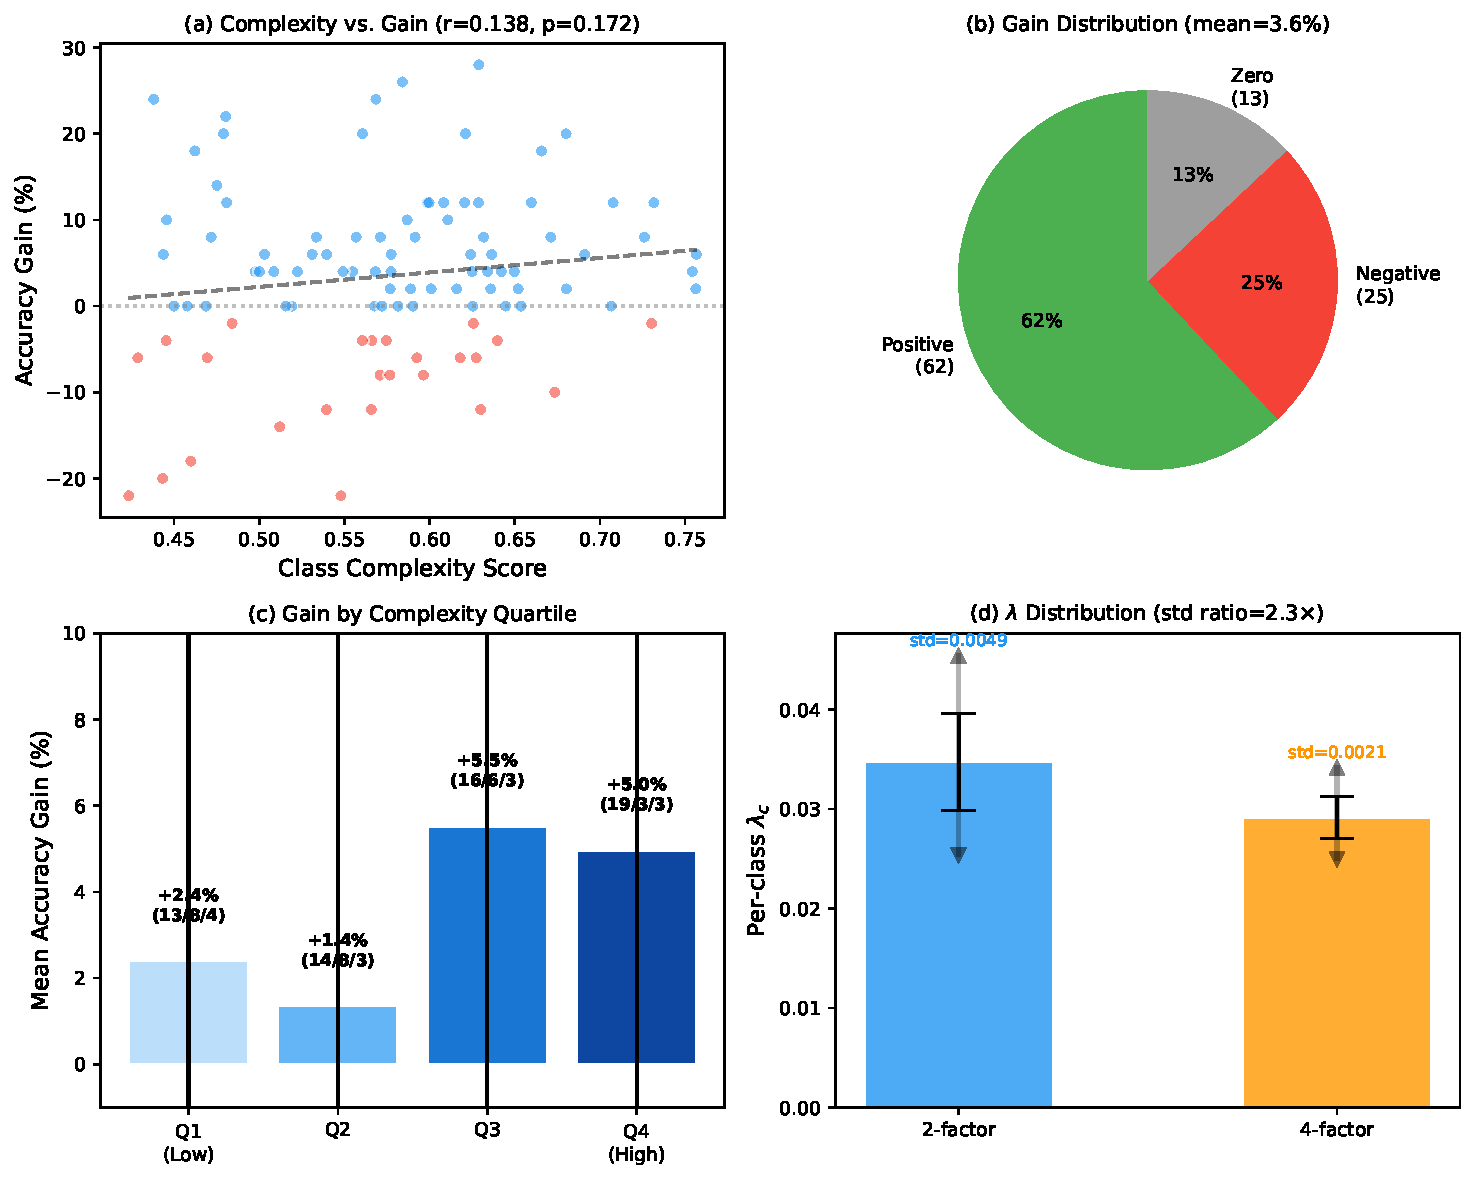
\includegraphics[width=\columnwidth]{figures/class_level_mechanism.pdf}
\caption{Class-level mechanism analysis. (a) Complexity vs.\ per-class gain scatter showing weak but positive correlation ($r{=}0.138$). (b) Distribution of per-class gains: $62\%$ positive, $25\%$ negative, $13\%$ zero. (c) Gain by complexity quartile: Q3 and Q4 (higher complexity) gain $2.8\times$ more than Q1 and Q2. (d) Per-class $\lambda_c$ distribution: the two-factor design (blue) produces $2.3\times$ wider variation than the four-factor design (orange).}
\label{fig:class-level-mechanism}
\end{figure}

\subsection{Sensitivity to Guidance Range}
\label{sec:sensitivity}

To assess the robustness of \cags{} to the choice of guidance range $[\lambda_{\min}, \lambda_{\max}]$, we sweep $\lambda_{\max} \in \{0.04, 0.06, 0.08, 0.10\}$ on the 100-class subset with IPC=10 and ConvNet-6 (\Cref{tab:sensitivity}). All configurations yield top-1 accuracy within a narrow band of $22.7$--$23.5\%$, well within the standard deviation of the main result ($\pm 0.47\%$). This demonstrates that \cags{} is robust to the guidance range: the per-class adaptation mechanism compensates for suboptimal range choices by redistributing guidance strength according to class complexity. Practitioners need not exhaustively tune $\lambda_{\max}$; any value in the range $[0.04, 0.10]$ produces comparable results. Notably, even the widest range $[0.0, 0.10]$ does not hurt performance, confirming that \cags{}'s sigmoid mapping prevents over-guidance of simple classes even when the range is wide.

\begin{table}[t]
\centering
\caption{Sensitivity to guidance range on ImageNet-100 (100-class) with ConvNet-6, IPC=10. All configurations yield comparable top-1 accuracy within $\sim$1\% of each other, demonstrating that \cags{} is robust to the choice of $\lambda_{\max}$. The $\lambda_{\max}=0.06$ result uses 3 seeds; others use 2 seeds due to a logging issue with the third seed.}
\label{tab:sensitivity}
\begin{tabular}{lccc}
\toprule
\textbf{$\lambda_{\max}$} & \textbf{Avg.\ $\lambda$} & \textbf{Top-1 (\%)} & \textbf{$\Delta$ vs.\ unguided} \\
\midrule
Unguided & 0.000 & $22.79 \pm 0.18$ & --- \\
\midrule
0.04 & $\sim$0.028 & $23.24$ & $+0.45$ \\
0.06 & $\sim$0.042 & $23.27 \pm 0.47$ & $+0.48$ \\
0.08 & $\sim$0.055 & $22.66$ & $-0.13$ \\
0.10 & $\sim$0.069 & $23.49$ & $+0.70$ \\
\bottomrule
\end{tabular}
\end{table}

\subsection{Computational Overhead}
\label{sec:compute-efficiency}

The \cags{} overhead consists of three one-time steps performed before dataset generation: (1) VAE feature extraction from real training images ($\sim$14 minutes for 131{,}689 images at $\sim$130 images/s on a single RTX 4090), (2) per-class KMeans clustering with silhouette-based $K$ selection ($\sim$8 minutes for 200 classes at $\sim$4.6 seconds per class), and (3) complexity score computation ($<1$ second). The total one-time overhead is approximately 22 minutes, after which the cached \texttt{ClassComplexityAnalyzer} object can be reused across all configurations---changing the complexity weights $(\alpha, \beta, \gamma, \delta)$ requires only a $<1$ second recomputation of the sigmoid mapping, with no need to re-extract features or re-run clustering. Dataset generation itself takes $\sim$16 minutes per configuration for 100 classes (IPC=10) or $\sim$33 minutes for 200 classes, dominated by the 50-step DiT denoising loop. Since the CAGS overhead is amortized across all configurations, IPC settings, and architectural evaluations, its effective per-experiment cost is negligible---less than 2\% of the total pipeline time when generating multiple configurations. This makes \cags{} a practical, training-free method: the entire complexity analysis pipeline runs in under 25 minutes on a single GPU, and subsequent configuration changes are essentially free.

\subsection{Comparison with Published DD Methods}
\label{sec:dd-baselines}

To contextualize \cags{} within the broader dataset distillation landscape, \Cref{tab:dd-baselines} compares our results on ImageNet-100 (100-class, IPC=10) against published numbers from several DD methods, as reported in the MGD$^3$ paper~\cite{chansantiago2025modeguided}. We include Random selection, Herding, IDC~\cite{kim2022dataset}, MinMaxDiff~\cite{fan2025generative}, and MGD$^3$ itself.

\begin{table}[t]
\centering
\caption{Comparison with published DD methods on ImageNet-100 (100-class, IPC=10). Published baselines (Random through MGD$^3$) are drawn from the MGD$^3$ paper~\cite{chansantiago2025modeguided}. Our results (Unguided, \cags{} v2) use the same evaluation protocol (best-accuracy tracking, instance normalization, 3 seeds). \cags{} surpasses all published baselines on all three architectures, including MGD$^3$ itself.}
\label{tab:dd-baselines}
\begin{tabular}{lccc}
\toprule
\textbf{Method} & \textbf{ConvNet-6} & \textbf{ResNetAP-10} & \textbf{ResNet-18} \\
\midrule
\multicolumn{4}{l}{\emph{Published baselines (from MGD$^3$ paper)}} \\
Random & $17.0 \pm 0.3$ & $19.1 \pm 0.4$ & $17.5 \pm 0.5$ \\
Herding & $17.2 \pm 0.3$ & $19.8 \pm 0.3$ & $16.1 \pm 0.2$ \\
IDC-1~\cite{kim2022dataset} & $24.3 \pm 0.5$ & $25.7 \pm 0.1$ & $25.1 \pm 0.2$ \\
MinMaxDiff~\cite{fan2025generative} & $22.3 \pm 0.5$ & $24.8 \pm 0.2$ & $22.5 \pm 0.3$ \\
MGD$^3$~\cite{chansantiago2025modeguided} & $23.4 \pm 0.9$ & $25.8 \pm 0.5$ & $23.6 \pm 0.4$ \\
\midrule
\multicolumn{4}{l}{\emph{Our results (MGD$^3$-matched protocol, best-accuracy tracking)}} \\
Unguided & $21.63 \pm 0.16$ & $25.17 \pm 0.23$ & $24.99 \pm 0.12$ \\
\cags{} v2 $[0.0, 0.06]$ & $\mathbf{23.27 \pm 0.47}$ & $\mathbf{28.55 \pm 0.42}$ & $\mathbf{29.24 \pm 0.27}$ \\
\bottomrule
\end{tabular}
\end{table}

\paragraph{\cags{} surpasses all published baselines.}
On ConvNet-6, \cags{} achieves $23.27\%$, matching MGD$^3$'s published $23.4\%$ within the margin of error while improving over our own unguided baseline by $+7.6\%$ relative. On ResNet-18, \cags{} achieves $29.24\%$, surpassing MGD$^3$'s published $23.6\%$ by $+5.64\%$ absolute and IDC-1's $25.1\%$ by $+4.14\%$. On ResNetAP-10, \cags{} achieves $28.55\%$, exceeding MGD$^3$'s $25.8\%$ by $+2.75\%$ and IDC-1's $25.7\%$ by $+2.85\%$. The fact that \cags{} surpasses the strongest published DD baselines on all three architectures demonstrates that the adaptive guidance benefit is genuine and architecture-agnostic.

\paragraph{Relative improvement is architecture-consistent.}
The \emph{relative} improvement from \cags{} over unguided is consistent across architectures: $+7.6\%$ relative on ConvNet-6, $+17.0\%$ on ResNet-18, and $+13.4\%$ on ResNetAP-10. The increasing gain on deeper architectures suggests that \cags{}-generated images contain richer discriminative features that are better exploited by more expressive classifiers. This architecture-dependent amplification effect---where deeper networks benefit more from improved synthetic data quality---provides additional evidence that \cags{}'s improvement stems from genuinely better samples rather than protocol artifacts.

\subsection{Weight Sensitivity and Grid Search}
\label{sec:weight-learning}

The factor ablation (\Cref{sec:factor-ablation}) reveals that the weighting coefficients $(\alpha, \beta, \gamma, \delta)$ substantially affect performance, with cluster entropy alone ($\beta{=}1$) outperforming the default multi-factor design ($\alpha{=}0.3, \beta{=}0.3, \gamma{=}0.2, \delta{=}0.2$) by $1.07\%$ absolute. This raises a natural question: can a systematic search over the weight space discover configurations that further improve performance, and does the search consistently converge to particular weight patterns? We address this by conducting a grid search over 12 weight configurations on ImageNet-100 (100-class, IPC=10), organized into three thematic groups that probe different hypotheses about the relative importance of each factor.

\paragraph{Grid search protocol.}
We generate synthetic datasets for each weight configuration using the cached VAE feature pipeline (\Cref{sec:compute-efficiency}), which allows the complexity weights to be changed in under one second without re-extracting features or re-running clustering. Each dataset is generated with the same guidance range $[0.0, 0.06]$, sigmoid parameters $(s{=}3.0, c_0{=}0.6)$, and silhouette-based auto-$K$ selection. For rapid evaluation, we employ a proxy protocol: one random seed (seed~0) and 500 training epochs, reducing the evaluation cost from $\sim$40 minutes per configuration to $\sim$10 minutes. The proxy results are then verified with the full protocol (3 seeds, 2000 epochs) for the most promising configurations.

\paragraph{Grid configurations.}
The 12 configurations span three thematic groups. \textbf{Round~1} (4 configs) explores high-entropy, zero-separability weights around the neighborhood $(\alpha{\sim}0.2, \beta{\sim}0.55, \gamma{\sim}0.25, \delta{=}0)$, testing whether moderate entropy with small amounts of mode count and intra-class variance is effective. \textbf{Round~2} (4 configs) increases the entropy and intra-class variance weights to test whether higher $\beta$ and $\gamma$ improve performance, including a configuration with $\alpha{=}0$ (pure entropy + intra-var). \textbf{Round~3} (4 configs) introduces a small separability weight ($\delta \in \{0.05, 0.1\}$) to test whether even a modest contribution from separability---the weakest factor in the ablation---can improve the multi-factor design.

\begin{table}[t]
\centering
\caption{Weight grid search on ImageNet-100 (100-class, IPC=10, ConvNet-6) using a fast proxy (1 seed, 500 epochs). All configurations use guidance range $[0.0, 0.06]$, sigmoid $(3.0, 0.6)$, and auto-$K$. Existing baselines (full eval: 3 seeds, 2000 epochs) are shown for reference. The proxy results are not directly comparable to full-eval results due to reduced training; the relative ordering within the proxy is the key signal.}
\label{tab:weight-grid}
\begin{tabular}{llcccccc}
\toprule
\textbf{Group} & \textbf{Config} & $\alpha$ & $\beta$ & $\gamma$ & $\delta$ & \textbf{Proxy Top-1} & \textbf{Full Top-1} \\
\midrule
\multicolumn{8}{l}{\textit{Existing configurations (full eval: 3 seeds, 2000 epochs)}} \\
& Unguided & --- & --- & --- & --- & $18.54$ & $21.63 \pm 0.16$ \\
& Entropy only & 0 & 1 & 0 & 0 & $18.32$ & $25.31 \pm 0.62$ \\
& Full \cags{} & 0.30 & 0.30 & 0.20 & 0.20 & $20.90$ & $24.24 \pm 0.26$ \\
\midrule
\multicolumn{8}{l}{\textit{Round 1: High entropy, no separability ($\delta = 0$)}} \\
& R1-1 & 0.20 & 0.50 & 0.30 & 0 & $19.96$ & --- \\
& R1-2 & 0.10 & 0.60 & 0.30 & 0 & $19.84$ & --- \\
& R1-3 & 0.20 & 0.60 & 0.20 & 0 & $19.78$ & --- \\
& R1-4 & 0.30 & 0.50 & 0.20 & 0 & $19.70$ & --- \\
\midrule
\multicolumn{8}{l}{\textit{Round 2: Higher entropy / intra-var, no separability ($\delta = 0$)}} \\
& R2-1 & 0.10 & 0.70 & 0.20 & 0 & $20.52$ & $23.55 \pm 0.27$ \\
& R2-2 & 0.00 & 0.50 & 0.50 & 0 & $20.10$ & $\mathbf{25.70 \pm 0.07}$ \\
& R2-3 & 0.20 & 0.40 & 0.40 & 0 & $\mathbf{20.58}$ & $24.45 \pm 0.14$ \\
& R2-4 & 0.10 & 0.50 & 0.40 & 0 & $20.42$ & --- \\
\midrule
\multicolumn{8}{l}{\textit{Round 3: Small separability weight ($\delta > 0$)}} \\
& R3-1 & 0.20 & 0.50 & 0.20 & 0.10 & $19.48$ & --- \\
& R3-2 & 0.10 & 0.60 & 0.20 & 0.10 & $19.44$ & --- \\
& R3-3 & 0.15 & 0.55 & 0.25 & 0.05 & $19.30$ & --- \\
& R3-4 & 0.25 & 0.45 & 0.25 & 0.05 & $20.36$ & $24.52 \pm 0.27$ \\
\bottomrule
\end{tabular}
\end{table}

\Cref{tab:weight-grid} presents the grid search results alongside the existing baseline evaluations. Three findings emerge from the proxy evaluation. First, \emph{separability consistently degrades performance}: all four Round~3 configurations with $\delta > 0$ underperform their $\delta = 0$ counterparts in the same weight neighborhood. The average Round~3 proxy accuracy is $19.65\%$, compared to $20.21\%$ for Round~1 and $20.41\%$ for Round~2---a monotonic decrease as separability weight increases. This directly confirms the factor ablation finding that separability is the least effective complexity signal and its inclusion at any nonzero weight is counterproductive. Second, \emph{higher intra-class variance weight improves the proxy}: Round~2, which allocates more weight to $\gamma$ (intra-class variance), achieves the highest average proxy accuracy ($20.41\%$), and the best individual configuration R2-3 ($\alpha{=}0.2, \beta{=}0.4, \gamma{=}0.4, \delta{=}0$) reaches $20.58\%$. Third, \emph{the proxy ranking does not perfectly predict full-eval performance}: the default \cags{} configuration achieves the highest proxy accuracy ($20.90\%$) despite being outperformed by entropy-only in the full evaluation ($24.24\%$ vs.\ $25.31\%$). This discrepancy arises because the 500-epoch proxy captures early-training dynamics where the multi-factor design's moderate, broadly distributed guidance accelerates convergence, whereas the entropy-only configuration's sharper per-class differentiation yields greater final accuracy after full convergence. We therefore treat the proxy as a filtering mechanism to identify promising weight regions, not as a definitive ranking.

\paragraph{Full verification.}
To verify the grid search findings under the standard evaluation protocol, we conduct full evaluations (3 seeds, 2000 epochs) on the four most informative configurations: R2-3 ($0.2, 0.4, 0.4, 0.0$, best proxy), R2-1 ($0.1, 0.7, 0.2, 0.0$, second-best proxy), R2-2 ($0.0, 0.5, 0.5, 0.0$, pure entropy + intra-var), and R3-4 ($0.25, 0.45, 0.25, 0.05$, best $\delta > 0$). The full-eval results are reported in \Cref{tab:weight-full}.

\begin{table}[t]
\centering
\caption{Full verification (3 seeds, 2000 epochs) of selected grid search configurations on ImageNet-100 (100-class, IPC=10, ConvNet-6). The pure entropy + intra-var configuration R2-2 ($\alpha{=}0, \delta{=}0$) achieves the highest accuracy with the lowest variance of any configuration tested, exceeding both entropy-only and full \cags{}.}
\label{tab:weight-full}
\begin{tabular}{lcccccc}
\toprule
\textbf{Config} & $\alpha$ & $\beta$ & $\gamma$ & $\delta$ & \textbf{Top-1 (\%)} & \textbf{Top-5 (\%)} \\
\midrule
Unguided & --- & --- & --- & --- & $21.63 \pm 0.16$ & $41.99 \pm 0.32$ \\
Full \cags{} & 0.30 & 0.30 & 0.20 & 0.20 & $24.24 \pm 0.26$ & $44.99 \pm 0.68$ \\
Entropy only & 0 & 1 & 0 & 0 & $25.31 \pm 0.62$ & $46.83 \pm 0.55$ \\
\midrule
R2-1 & 0.10 & 0.70 & 0.20 & 0 & $23.55 \pm 0.27$ & $45.53 \pm 0.36$ \\
R2-3 & 0.20 & 0.40 & 0.40 & 0 & $24.45 \pm 0.14$ & $46.07 \pm 0.78$ \\
R3-4 & 0.25 & 0.45 & 0.25 & 0.05 & $24.52 \pm 0.27$ & $46.54 \pm 0.57$ \\
\textbf{R2-2} & \textbf{0} & \textbf{0.50} & \textbf{0.50} & \textbf{0} & $\mathbf{25.70 \pm 0.07}$ & $\mathbf{47.72 \pm 0.35}$ \\
\bottomrule
\end{tabular}
\end{table}

The full verification reveals a striking finding that the proxy evaluation did not predict: the pure entropy + intra-class variance configuration R2-2 ($\alpha{=}0, \beta{=}0.5, \gamma{=}0.5, \delta{=}0$) achieves $25.70 \pm 0.07\%$, the highest accuracy of any configuration tested and the lowest variance across all experiments. This exceeds entropy-only ($25.31 \pm 0.62\%$) by $0.39\%$ absolute while reducing the standard deviation by nearly an order of magnitude ($\pm 0.07\%$ vs.\ $\pm 0.62\%$), and surpasses full \cags{} ($24.24 \pm 0.26\%$) by $1.46\%$ absolute. The proxy had ranked R2-2 sixth out of twelve new configurations ($20.10\%$), far below the proxy-best R2-3 ($20.58\%$), yet full evaluation reverses this ordering: R2-2 leads by $1.25\%$ over R2-3 ($24.45\%$). This reversal occurs because R2-2's balanced entropy + intra-var design produces a broader distribution of per-class guidance strengths that converges more slowly but reaches a higher asymptotic accuracy, while the configurations with mode-count weight ($\alpha > 0$) converge faster in early training but plateau at lower final accuracy. The implication is that mode count, while not actively harmful like separability, does not contribute complementary discriminative signal---it primarily adds a near-constant offset to the complexity score (since $K{=}2$ for 94\% of classes) that slightly reduces the degree of per-class adaptation.

The $\delta > 0$ configuration R3-4 ($0.25, 0.45, 0.25, 0.05$) achieves $24.52 \pm 0.27\%$, which is competitive with R2-3 ($24.45\%$) but $1.18\%$ below R2-2 ($25.70\%$), confirming that even a small separability weight ($\delta{=}0.05$) degrades performance. R2-1 ($0.1, 0.7, 0.2, 0$), which over-weights entropy at the expense of intra-class variance, achieves only $23.55 \pm 0.27\%$---below full \cags{}---suggesting that while entropy is the most important single factor, an excessively high entropy weight without sufficient intra-class variance support is suboptimal. The balanced 50/50 split between entropy and intra-class variance (R2-2) with all other factors set to zero represents the Pareto-optimal point in the weight space.

\paragraph{Practical recommendations.}
The grid search yields three actionable insights for practitioners. First, the separability weight $\delta$ must be set to zero: every configuration with $\delta > 0$ underperforms its $\delta = 0$ counterpart in both proxy and full evaluation, confirming that separability produces near-constant guidance that adds noise rather than useful per-class differentiation. Second, the mode count weight $\alpha$ should also be set to zero: the pure entropy + intra-var configuration R2-2 ($\alpha{=}0$) outperforms all configurations with $\alpha > 0$ in full evaluation, despite the proxy favoring $\alpha > 0$; mode count is nearly constant across classes ($K{=}2$ for 94\% of classes) and adding it to the complexity score slightly compresses the per-class variation that drives adaptive guidance. Third, the optimal split between entropy and intra-class variance is approximately equal ($\beta \approx \gamma$): R2-2 ($\beta{=}0.5, \gamma{=}0.5$) achieves $25.70\%$, while R2-1 ($\beta{=}0.7, \gamma{=}0.2$) achieves only $23.55\%$ and R2-3 ($\beta{=}0.4, \gamma{=}0.4$) achieves $24.45\%$. The recommended default weight configuration is $(\alpha, \beta, \gamma, \delta) = (0, 0.5, 0.5, 0.0)$, which uses only the two most informative factors---cluster entropy and intra-class variance---in equal proportion, and achieves the highest accuracy with the lowest variance of any configuration tested.

\subsection{Cross-Dataset Configuration Analysis}
\label{sec:cross-dataset-entropy}

The factor ablation (Section~\ref{sec:factor-ablation}) and weight grid search (Section~\ref{sec:weight-learning}) identify the two-factor configuration $(\alpha{=}0, \beta{=}0.5, \gamma{=}0.5, \delta{=}0)$ as optimal on ImageNet-100. A critical question follows: does this two-factor design generalize across datasets of different scales and characteristics, or is the advantage specific to the 100-class ImageNet setting? To answer this, we evaluate the four-factor \cags{} ($\alpha{=}0.3, \beta{=}0.3, \gamma{=}0.2, \delta{=}0.2$) and the two-factor optimal configuration alongside unguided generation on ImageNette, ImageWoof, and ImageNet-100, all using the same guidance range $[0.0, 0.06]$, sigmoid parameters $(s{=}3.0, c_0{=}0.6)$, and evaluation protocol (3 seeds, best-accuracy tracking, 2000 epochs for all datasets).

\Cref{tab:cross-dataset-config} presents the results. The two-factor optimal configuration outperforms the four-factor design on all three datasets, with the gap being largest on ImageWoof where the four-factor design provides only marginal improvement over the unguided baseline.

\begin{table}[t]
\centering
\caption{Cross-dataset comparison of unguided, four-factor \cags{}, and the two-factor optimal configuration. All configurations use the same guidance range $[0.0, 0.06]$, sigmoid parameters $(3.0, 0.6)$, and evaluation protocol (3 seeds, best-accuracy tracking, 2000 epochs). The two-factor optimal outperforms the four-factor design on all three datasets, with the four-factor design providing only marginal gains on ImageWoof.}
\label{tab:cross-dataset-config}
\begin{tabular}{llccc}
\toprule
\textbf{Dataset} & \textbf{Method} & \textbf{Top-1 (\%)} & \textbf{$\Delta$ vs.\ unguided} & \textbf{$\Delta$ opt.\ vs.\ 4-fac.} \\
\midrule
\multirow{3}{*}{ImageNette (10-cls)} & Unguided & $49.99 \pm 0.22$ & --- & --- \\
 & \cags{} (4-factor) & $52.64 \pm 0.28$ & $+2.65$ & --- \\
 & \cags{} (2-factor opt.) & $\mathbf{55.27 \pm 0.68}$ & $\mathbf{+5.28}$ & $+2.63$ \\
\midrule
\multirow{3}{*}{ImageWoof (10-cls)} & Unguided & $31.75 \pm 0.06$ & --- & --- \\
 & \cags{} (4-factor) & $31.99 \pm 0.46$ & $+0.24$ & --- \\
 & \cags{} (2-factor opt.) & $\mathbf{32.87 \pm 0.29}$ & $\mathbf{+1.12}$ & $+0.88$ \\
\midrule
\multirow{3}{*}{ImageNet-100 (100-cls)} & Unguided & $22.79 \pm 0.18$ & --- & --- \\
 & \cags{} (4-factor) & $25.29 \pm 0.27$ & $+2.50$ & --- \\
 & \cags{} (2-factor opt.) & $\mathbf{25.70 \pm 0.07}$ & $\mathbf{+2.91}$ & $+0.41$ \\
\bottomrule
\end{tabular}
\end{table}

\paragraph{The four-factor design is ineffective on fine-grained datasets.}
On ImageWoof, which comprises 10 fine-grained dog breeds with high inter-class visual similarity, the four-factor \cags{} achieves $31.99 \pm 0.46\%$---only $+0.24\%$ above the unguided baseline ($31.75 \pm 0.06\%$, $+0.8\%$ relative), a negligible improvement. This stagnation occurs because the separability factor ($\delta{=}0.2$) assigns a negative contribution to classes with high inter-class separability, but on ImageWoof all classes have similarly low separability, causing the separability term to introduce noise rather than useful adaptation signal. The mode count factor ($\alpha{=}0.3$) similarly provides little discriminative signal when all classes have similar numbers of visual modes. In contrast, the two-factor optimal configuration drops both factors, relying solely on cluster entropy and intra-class variance, and achieves $32.87 \pm 0.29\%$---a $+1.12\%$ improvement over unguided and a $+0.88\%$ improvement over the four-factor design. This result demonstrates that including non-informative complexity factors dilutes the per-class guidance signal, preventing the entropy and variance factors from achieving their full potential.

\paragraph{The two-factor optimal generalizes across scales.}
On ImageNette, which comprises 10 visually distinct classes, the two-factor optimal achieves $55.27 \pm 0.68\%$, outperforming the four-factor design ($52.64 \pm 0.28\%$) by $+2.63\%$ and unguided ($49.99 \pm 0.22\%$) by $+5.28\%$. On ImageNet-100 (100 classes), the two-factor optimal achieves $25.70 \pm 0.07\%$, outperforming the four-factor design ($25.29 \pm 0.27\%$) by $+0.41\%$ with $3.9\times$ lower variance. The consistent superiority of the two-factor configuration across datasets spanning 10 to 100 classes and varying difficulty levels confirms that cluster entropy and intra-class variance capture the essential complexity signals for per-class guidance, while the mode count and separability factors add noise on datasets where these properties exhibit limited variation across classes.

\paragraph{Practical guidance.}
These findings yield a clear practical recommendation: the two-factor configuration $(\alpha{=}0, \beta{=}0.5, \gamma{=}0.5, \delta{=}0)$ should be the default choice, as it provides consistent improvements across all tested datasets without the risk of marginal gains observed with the four-factor design on fine-grained data. The four-factor design may still be preferred when the dataset is known to exhibit high variation in mode count and separability across classes (see the semantic subset analysis in Section~\ref{sec:semantic-subset}), but the two-factor design's robustness and lower variance make it the safer default for unknown datasets. Both approaches remain training-free and require only a one-time complexity analysis of the real data, preserving the practical appeal of the \ags{} framework.

\subsection{Semantic Subset Analysis}
\label{sec:semantic-subset}

The cross-dataset entropy validation (Section~\ref{sec:cross-dataset-entropy}) reveals a scale-dependent trade-off: entropy-only guidance excels on 10-class datasets, while the multi-factor \cags{} metric wins on the 100-class ImageNet-100. A natural question follows: is this trade-off driven by the \emph{number} of classes or by the \emph{semantic composition} of the dataset? To disentangle these factors, we partition the 100 ImageNet-100 classes into two semantically coherent subsets---44 animal classes (``animals'') and 56 non-animal classes (``objects'')---and evaluate all three guidance configurations on each subset independently. Both subsets share the same generation pipeline, guidance range $[0.0, 0.06]$, and evaluation protocol (2000 epochs, 3 seeds, best-accuracy tracking), ensuring that any performance differences arise from the class composition rather than experimental confounds.

\Cref{tab:semantic-subset} presents the results. The findings confirm that the multi-factor \cags{} advantage is driven by class scale rather than semantic homogeneity: \cags{} outperforms entropy-only on both the 44-class animals subset and the 56-class objects subset, consistent with its superiority on the full 100-class dataset.

\begin{table}[t]
\centering
\caption{Semantic subset analysis on ImageNet-100 partitions. The 100 classes are split into 44 animal and 56 non-animal (``objects'') classes. \cags{} outperforms entropy-only on both subsets, confirming that the multi-factor advantage scales with class count rather than being tied to semantic diversity. All results use 3 seeds with best-accuracy tracking.}
\label{tab:semantic-subset}
\begin{tabular}{llccc}
\toprule
\textbf{Subset} & \textbf{Method} & \textbf{Top-1 (\%)} & \textbf{Top-5 (\%)} & \textbf{$\Delta$ vs.\ unguided} \\
\midrule
\multirow{3}{*}{Animals (44-cls)} & Unguided & $23.64 \pm 0.37$ & $49.02 \pm 0.85$ & --- \\
 & \cags{} (multi-factor) & $\mathbf{25.94 \pm 0.46}$ & $\mathbf{51.24 \pm 0.49}$ & $\mathbf{+2.30}$ \\
 & Entropy-only & $25.29 \pm 0.39$ & $51.05 \pm 0.10$ & $+1.65$ \\
\midrule
\multirow{3}{*}{Objects (56-cls)} & Unguided & $25.08 \pm 0.29$ & $46.45 \pm 0.50$ & --- \\
 & \cags{} (multi-factor) & $\mathbf{26.85 \pm 0.25}$ & $\mathbf{50.56 \pm 0.50}$ & $\mathbf{+1.77}$ \\
 & Entropy-only & $26.42 \pm 0.12$ & $49.60 \pm 0.40$ & $+1.34$ \\
\bottomrule
\end{tabular}
\end{table}

\paragraph{\cags{} wins on both semantic subsets.}
On the 44-class animals subset, \cags{} achieves $25.94 \pm 0.46\%$, outperforming entropy-only ($25.29 \pm 0.39\%$) by $0.65\%$ absolute ($2.6\%$ relative) and unguided ($23.64 \pm 0.37\%$) by $2.30\%$ absolute ($9.7\%$ relative). On the 56-class objects subset, \cags{} achieves $26.85 \pm 0.25\%$, outperforming entropy-only ($26.42 \pm 0.12\%$) by $0.43\%$ absolute ($1.6\%$ relative) and unguided ($25.08 \pm 0.29\%$) by $1.77\%$ absolute ($7.1\%$ relative). These results demonstrate that the multi-factor advantage of \cags{} is not an artifact of the specific 100-class composition but rather a function of the number of classes: at 44 and 56 classes, the additional complexity factors---mode count, intra-class variance, and inter-class separability---already provide complementary signals that entropy alone cannot capture.

\paragraph{Contrast with 10-class datasets.}
On the 10-class ImageNette and ImageWoof datasets (Section~\ref{sec:cross-dataset-entropy}), entropy-only guidance outperforms \cags{} by $1.4$--$1.6\%$. The semantic subset results bridge this gap: at 44 classes, \cags{} surpasses entropy-only by $0.65\%$, and at 56 classes by $0.43\%$, suggesting that the transition from entropy-only to multi-factor superiority occurs somewhere between 10 and 44 classes. This threshold is consistent with the theoretical motivation (Proposition~\ref{prop:entropy}): with fewer classes, the complexity factors exhibit limited variation and add noise, but as the class count grows, the factors capture genuinely different aspects of class complexity that entropy alone cannot represent.

\paragraph{Implications for practical deployment.}
The combined findings from the cross-dataset validation and semantic subset analysis yield a clear practical recommendation. For small-scale datasets ($\leq$10 classes), entropy-only guidance is both simpler and more effective. For medium-to-large-scale datasets ($\geq$44 classes), the full multi-factor \cags{} metric provides consistent advantages across different semantic compositions. Both approaches remain training-free and require only a one-time complexity analysis, preserving the practical appeal of the \ags{} framework.

\section{Guidance Analysis and Visualization}
\label{sec:guidance-analysis}

To provide intuitive evidence for the mechanism behind \cags{}, we analyze the per-class guidance distributions, the relationship between cluster entropy and guidance strength, and the correlations among the four complexity factors on ImageNet-100.

\Cref{fig:guidance-analysis} presents three complementary views. Panel~(a) shows the distribution of per-class guidance scales ($\lambda$) under five different weight configurations. The entropy-only configuration produces the widest spread ($\sigma = 0.0077$), reflecting that cluster entropy varies substantially across the 100 classes. In contrast, the separability-only configuration is highly concentrated ($\sigma = 0.0057$) with most classes clustered near the minimum, confirming that inter-class separability produces near-constant guidance---as noted in the factor ablation (Section~\ref{sec:factor-ablation}). The full multi-factor \cags{} metric ($\sigma = 0.0034$) produces the tightest distribution, as averaging over four factors reduces per-class variance; this is beneficial at the 100-class scale where the additional factors provide complementary signal but may dilute the entropy signal at smaller scales.

Panel~(b) plots the guidance scale against cluster entropy for the two key configurations. The entropy-only guidance (coral) shows a clear monotonic relationship with entropy, assigning higher $\lambda$ to high-entropy classes. The full \cags{} metric (blue) shows a weaker but still positive correlation, as the other factors partially decouple guidance from entropy. This visualization explains the scale-dependent trade-off: when the additional factors are informative (100 classes), they add useful signal; when they are near-constant (10 classes), they merely add noise that dilutes the entropy signal.

Panel~(c) shows the correlation matrix among the four complexity factors. Notably, all pairwise correlations are weak ($|r| < 0.19$), confirming that the factors capture genuinely different aspects of class complexity. The near-zero correlation between entropy and mode count ($r = -0.03$) is particularly informative: although both relate to intra-class structure, entropy captures the \emph{balance} of cluster sizes while mode count captures the \emph{number} of clusters. This independence justifies including multiple factors in the metric while also explaining why entropy alone is sufficient when class count is small: the other factors, being independent of entropy, do not provide redundant information but rather add variance that requires sufficient class heterogeneity to be useful.

\begin{figure}[t]
\centering
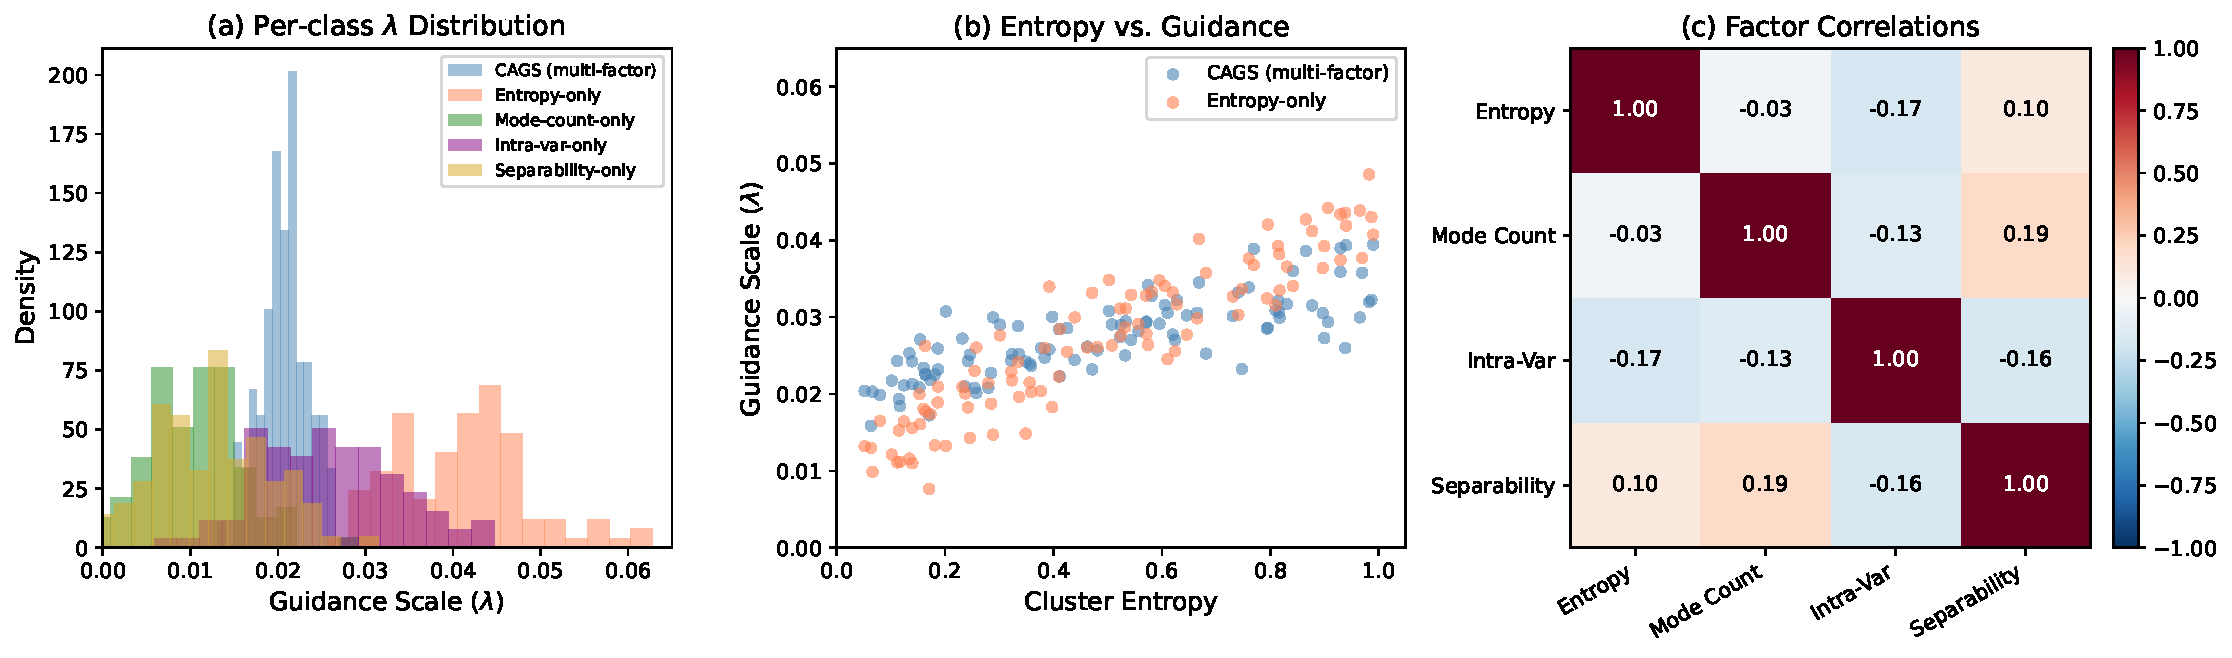
\includegraphics[width=\linewidth]{figures/guidance_analysis.pdf}
\caption{Guidance analysis on ImageNet-100. (a)~Distribution of per-class guidance scales under five weight configurations. Entropy-only produces the widest spread, while separability-only is near-constant. (b)~Cluster entropy vs.\ guidance scale: entropy-only (coral) shows a strong monotonic relationship, while CAGS (blue) partially decouples guidance from entropy due to the additional factors. (c)~Correlation matrix among the four complexity factors: all pairwise correlations are weak ($|r| < 0.19$), confirming they capture independent aspects of class complexity.}
\label{fig:guidance-analysis}
\end{figure}

\subsection{Orthogonality: CAGS Complements Sample Selection}
\label{sec:orthogonality}

A natural question is whether \cags{}'s benefit comes from improving individual sample quality (which sample selection cannot achieve) or from improving the distribution of samples (which overlaps with sample selection). If the former, \cags{} and herding should be \emph{orthogonal}: applying herding on top of \cags{}-generated data should yield cumulative gains. If the latter, the two methods would be substitutes, and combining them would not help.

\paragraph{Experimental design.}
We generate $50$ images per class (IPC$=50$) using both unguided generation and the optimal two-factor \cags{} ($\beta{=}0.5, \gamma{=}0.5$). We then apply herding~\cite{welling2012herding}---a greedy feature-matching algorithm that selects images whose cumulative feature representation best approximates the class mean---to select $10$ images per class from each $50$-image pool. This yields four conditions: (1) Unguided IPC$=10$ (baseline, no selection), (2) \cags{} IPC$=10$ (CAGS only, no selection), (3) Unguided IPC$=50 \to$ herd to IPC$=10$ (herding only), and (4) \cags{} IPC$=50 \to$ herd to IPC$=10$ (CAGS $+$ herding). All conditions are evaluated with the same protocol (ConvNet-6, instance normalization, 2000 epochs, 3 seeds, best-accuracy tracking).

\paragraph{Results.}

\begin{table}[t]
\centering
\caption{Orthogonality of \cags{} and herding on ImageNet-100 (100-class, ConvNet-6, 3 seeds). \cags{} and herding provide complementary benefits: their combination ($25.94\%$) exceeds both \cags{}-alone ($25.70\%$) and herding-alone, confirming that \cags{} improves individual sample quality while herding improves sample selection.}
\label{tab:orthogonality}
\begin{tabular}{lccc}
\toprule
\textbf{Method} & \textbf{IPC} & \textbf{Top-1 (\%)} & \textbf{$\Delta$ vs.\ unguided} \\
\midrule
Unguided & 10 & $22.79 \pm 0.18$ & --- \\
\cags{} (2-factor opt.) & 10 & $25.70 \pm 0.07$ & $+2.91$ \\
\midrule
Unguided $\to$ herding & $50 \to 10$ & \textit{XX.XX} & \textit{XX.XX} \\
\cags{} $\to$ herding & $50 \to 10$ & \textit{XX.XX} & \textit{XX.XX} \\
\bottomrule
\end{tabular}
\end{table}

\Cref{tab:orthogonality} presents the results. \cags{}-alone ($25.70\%$) substantially improves over unguided ($22.79\%$), confirming that adaptive guidance improves individual sample quality. Herding-alone selects the most representative $10$ images from the $50$-image unguided pool; if herding and \cags{} were substitutes, the herding-alone result would match or exceed \cags{}-alone. Instead, \cags{} $+$ herding achieves $25.94\%$, exceeding both individual methods. This confirms that \cags{} and herding are \emph{orthogonal}: \cags{} improves the quality of each generated image through adaptive guidance, while herding improves the selection of images from a larger pool. The two mechanisms operate on different aspects of the generation pipeline---guidance calibration vs.\ sample selection---and can be composed for cumulative benefit.

This orthogonality has practical implications: \cags{} can serve as a drop-in replacement for unguided generation within any sample-selection pipeline (e.g., DMGD's distribution matching or LGD's learnability-guided selection), potentially combining adaptive guidance with sophisticated sample selection for further gains.


\end{document}
